\section{Deployment of a Kubernetes cluster, using two selected methods}
\textit{This is a practical chapter and it was written together with performing the empirical work and writing the source code. Main steps of Kubernetes cluster deployment will be described. Also, encountered problems will be listed and potential solutions will be presented.}
\\

\subsection{Experimental deployments using Kops}
\textit{In this subsection first experiments of deploying a Kubernetes cluster with Kops on AWS are described.}
\\

TODO: write about current directory from which commands are run
TODO: write about common env variables set

\subsubsection{Deployment without prerequisite steps done}

Although the aim of this work is to create a production Kubernetes cluster, it is always welcome, when there is a possibility to start working with a program easily. It is nice to have a simple working proof of concept (POC). Thus, it was decided to start with Kops without performing any prerequisite steps. The following commands were invoked:
\begin{lstlisting}[basicstyle=\tiny,caption={Commands used to create a cluster with kops, without prerequisite steps performed},captionpos=b,language=Bash,xleftmargin=1cm]
$ export KOPS_STATE_STORE=s3://dummy-k8s-kops-state-store
$ export NAME=dummy-k8s-kops.k8s.local
$ kops create cluster --state "s3://${K8S_EXP_KOPS_S3_BUCKET}" \
--master-zones=eu-west-1a --master-count=1 --master-size=t2.nano \
--zones=eu-west-1a --node-count=1 --node-size=t2.nano \
${NAME}
\end{lstlisting}


The command \textit{kops create cluster} instructs kops how to create a cluster. The flag \textit{--master-count=1} says that there will be one master node created, \textit{--master-size=t2.nano} sets the EC2 instance type and \textit{--master-zones=eu-west-1a} configures the AZs in which master nodes will be deployed. Similar flags are used to configure worker nodes. The \textit{--state} flag sets which S3 bucket to use.  \textbf{As expected and what is aligned with the Kops documentation\cite{online-kops-aws}, the above commands failed}, because the S3 bucket was not created. The command failed with the following output:
\begin{lstlisting}[basicstyle=\tiny,caption={Output of the commands used to create a cluster with Kops, without prerequisite steps performed},captionpos=b,language=Bash,xleftmargin=1cm]
error reading cluster configuration "dummy-k8s-kops.k8s.local":
error reading s3://dummy-k8s-kops-state-store/dummy-k8s-kops.k8s.local/config:
Could not retrieve location for AWS bucket dummy-k8s-kops-state-store
\end{lstlisting}

The Kops documentation\cite{online-kops-aws} informs that the following goals should be first accomplished, before deploying a Kubernetes cluster:
\begin{itemize}
\item AWS CLI tools should be installed
\item AWS credentials should be set
\item AWS IAM user and its permissions should be set
\item DNS should be configured
\item An S3 bucket should be created for storing a cluster state
\item AWS Region and Availability Zones should be chosen
\end{itemize}

Further in this chapter, after all the prerequisites will have been met, Kops will be used to create a production Kubernetes cluster.

\subsubsection{Deployment with prerequisite steps done - first working cluster}

First, all the prerequisites were done and they are described here. In order to make things simpler, an AWS user with administrator permissions was used. SSH keypair was already set. Then, it was decided to use the gossip-based DNS. Then, an S3 bucket was created to keep the Kops cluster configuration. Both versioning and server side encryption of the S3 bucket were enabled. Versioning was strongly recommended, because thanks to it, one may revert or recover a previous cluster state store. S3 bucket encryption is not required, but may be needed for compliance reasons\cite{online-kops-aws}. \textbf{Setting the S3 bucket} was done by the following commands:
\begin{lstlisting}[basicstyle=\tiny,caption={Commands used to set an AWS S3 bucket for Kops},captionpos=b,language=Bash,xleftmargin=1cm]
$ export K8S_EXP_REGION="eu-west-1"
$ export K8S_EXP_KOPS_S3_BUCKET="k8s-kops-for-masters-thesis.k8s.local"
$ export K8S_EXP_ENVIRONMENT="testing"
$ export K8S_EXP_CLUSTER_NAME="${K8S_EXP_ENVIRONMENT}.${K8S_EXP_KOPS_S3_BUCKET}"
$ aws s3api create-bucket --bucket ${K8S_EXP_KOPS_S3_BUCKET} --region ${K8S_EXP_REGION} \
--create-bucket-configuration LocationConstraint=${K8S_EXP_REGION}
$ aws s3api put-bucket-versioning --bucket ${K8S_EXP_KOPS_S3_BUCKET} \
--versioning-configuration Status=Enabled
$ aws s3api put-bucket-encryption --bucket ${K8S_EXP_KOPS_S3_BUCKET} \
--server-side-encryption-configuration '{"Rules":[{"ApplyServerSideEncryptionByDefault":{"SSEAlgorithm":"AES256"}}]}'
\end{lstlisting}

Then, \textbf{the command below was used to make Kops create the cluster configuration and put it in the S3 bucket}. The command is presented below together with its output:
\begin{lstlisting}[basicstyle=\tiny,caption={Command used to make Kops create the cluster configuration and put it in the S3 bucket},captionpos=b,language=Bash,xleftmargin=1cm]
$ kops create cluster --state "s3://${K8S_EXP_KOPS_S3_BUCKET}" \
--master-zones=eu-west-1a --master-count=1 --master-size=t2.nano \
--zones=eu-west-1a --node-count=1 --node-size=t2.nano ${K8S_EXP_CLUSTER_NAME}

error building tasks: error remapping manifest addons/kops-controller.addons.k8s.io/k8s-1.16.yaml: \
error parsing yaml: error converting YAML to JSON: yaml: line 56: did not find expected alphabetic or numeric character
\end{lstlisting}

Running this command resulted in \textbf{a not successful exit status (1)}. The reason for this was that the development environment had a non-numeric environment variable set. It was a password and the variable value contained asterisks (\textit{****}). After the variable was unset (with the bash command: \textit{unset}), the \textit{kops create cluster} succeeded. The output of this command presented the list of actions which Kops will perform on the AWS account, e.g. creating EBS volumes for Etcd, configuring IAM, creating keypairs for Kubernetes services, configuring network and setting EC2 instances. Details of the to-be-created resources were also provided, for example, the command output informed that the EC2 image will be: \textit{kope.io/k8s-1.16-debian-stretch-amd64-hvm-ebs-2020-01-17}. Apart from printing the output, Kops created a directory named the same as the cluster name (\textit{testing.k8s-kops-for-masters-thesis.k8s.local}) in the S3 bucket. Among the files automatically created by Kops, there is a configuration file named: \textit{config} and it contains the cluster settings. \textbf{The cluster configuration can be edited from command line} with the command presented below. Running this command starts a vim session.
\begin{lstlisting}[basicstyle=\tiny,caption={Command used to edit a Kubernetes cluster managed by Kops},captionpos=b,language=Bash,xleftmargin=1cm]
$ kops edit cluster ${K8S_EXP_CLUSTER_NAME} --state "s3://${K8S_EXP_KOPS_S3_BUCKET}"
\end{lstlisting}
After editing the configuration, \textbf{the cluster can be created or updated} (if it was created earlier) with the next command. This command deploys a cluster on AWS and prints a helpful output. Part of the output is also attached below:
\begin{lstlisting}[basicstyle=\tiny,caption={Command used to deploy a Kubernetes cluster with Kops},captionpos=b,language=Bash,xleftmargin=1cm]
$ kops update cluster ${K8S_EXP_CLUSTER_NAME} --state "s3://${K8S_EXP_KOPS_S3_BUCKET}" --yes

# some output lines omitted
Cluster is starting.  It should be ready in a few minutes.

Suggestions:
 * validate cluster: kops validate cluster
 * list nodes: kubectl get nodes --show-labels
 * ssh to the master: ssh -i ~/.ssh/id_rsa admin@api.testing.k8s-kops-for-masters-thesis.k8s.local
 * the admin user is specific to Debian. If not using Debian please use the appropriate user based on your OS.
 * read about installing addons at: https://github.com/kubernetes/kops/blob/master/docs/operations/addons.md.
\end{lstlisting}

Unfortunately, the commands listed as suggestions above did not work. They resulted in:
\begin{lstlisting}[basicstyle=\tiny,caption={Commands run in attempt to connect with a cluster created by Kops together with returned output},captionpos=b,language=Bash,xleftmargin=1cm]
$ kops validate cluster ${K8S_EXP_CLUSTER_NAME} --state "s3://${K8S_EXP_KOPS_S3_BUCKET}"
Validating cluster testing.k8s-kops-for-masters-thesis.k8s.local
unexpected error during validation: error listing nodes: \
Get https://api-testing-k8s-kops-for--l9puut-394396927.eu-west-1.elb.amazonaws.com/api/v1/nodes: EOF

$ ssh -i ~/.ssh/id_rsa admin@api.testing.k8s-kops-for-masters-thesis.k8s.local
ssh: Could not resolve hostname api.testing.k8s-kops-for-masters-thesis.k8s.local: \
Name does not resolve
\end{lstlisting}

It was expected that the latter command should fail, because \textit{api.testing.k8s-kops-for-masters-thesis.k8s.local} is not a public domain name and thus, it is not available from remote locations (such as this work author's computer). But the former command should have worked. In practice, there was no way to connect to the EC2 instances. Thus, as a solution - bigger EC2 instances were used: \textit{t2.micro} instead of \textit{t2.micro}. Using this particular instance type, \textit{t2.micro}, was observed in several online sources\cite{online-ha-k8s-blog}\cite{online-perfect-k8s-blog}\cite{online-kops-sa}. This time the command succeeded. It was possible to list the worker nodes with: \textit{kubectl get nodes}. It was doable thanks to kops creating an AWS Classic LoadBalancer. It exposed the following DNS A record that was publicly reachable: \textit{api-testing-k8s-kops-for--l9puut-1371087518.eu-west-1.elb.amazonaws.com}.

It is also worth mentioning that the kubeconfig (\textit{~/.kube/config}), a Kubernetes configuration file needed to connect to a cluster, was generated automatically. Another thing to notice is that the command, which deploys a Kubernetes cluster, returned immediately, without waiting for the cluster to be ready. In the next deployments, some waiting mechanism must be applied, so that the cluster creation and verification can be automated. Below, there is a command used to request information about the cluster:
\begin{lstlisting}[basicstyle=\tiny,caption={Command used to request information about a running Kubernetes cluster},captionpos=b,language=Bash,xleftmargin=1cm]
$ kubectl cluster-info
Kubernetes master is running at https://api-testing-k8s-kops-for--l9puut-1371087518.eu-west-1.elb.amazonaws.com
KubeDNS is running at https://api-testing-k8s-kops-for--l9puut-1371087518.eu-west-1.elb.amazonaws.com/api/v1/namespaces/kube-system/services/kube-dns:dns/proxy

To further debug and diagnose cluster problems, use 'kubectl cluster-info dump'.
\end{lstlisting}

After the first cluster was successfully deployed, the following command was used in order export the cluster configuration into YAML file. It will be needed for production deployment.
\begin{lstlisting}[basicstyle=\tiny,caption={Command used to export a Kubernetes cluster configuration},captionpos=b,language=Bash,xleftmargin=1cm]
$ kops get -o yaml --name ${K8S_EXP_CLUSTER_NAME} --state "s3://${K8S_EXP_KOPS_S3_BUCKET}"
\end{lstlisting}

Then, \textbf{the cluster was deleted}. There were no problems with deleting the cluster. It took several minutes, but the following command succeeded and all the AWS resources (except for the manually created S3 bucket) were deleted:

\begin{lstlisting}[basicstyle=\tiny,caption={Command used to delete a Kubernetes cluster created with Kops},captionpos=b,language=Bash,xleftmargin=1cm]
$ kops delete cluster --name ${K8S_EXP_CLUSTER_NAME} --state "s3://${K8S_EXP_KOPS_S3_BUCKET}" --yes
\end{lstlisting}

The steps described in this section proved that it is possible to deploy a Kubernetes cluster on AWS with kops. It was a POC. The next cluster will attempt to satisfy the production deployment requirements.

%%%%%%%%%%%%%%%%%%%%%%%%%%%%%%%%%%%%%%%%%%%%%%%%%%%%%%%%%%%%%%%%%%%%%%%%%%%%%%%%
\subsection{Experimental deployments using eksctl}
\textit{In this subsection first experiments of deploying a Kubernetes cluster with eksctl on AWS are described.}
\\

In order to be consistent, the similar first experiment was performed using eksctl. It was decided to store the configuration locally in a YAML configuration file. The alternative was to set many command line flags. Below, \textbf{the configuration file and then the eksctl CLI command used to create a cluster are presented}:
\begin{lstlisting}[basicstyle=\tiny,caption={Commands used to create a cluster with eksctl, without prerequisite steps performed},captionpos=b,language=Bash,xleftmargin=1cm]
$ cat cluster.yaml
apiVersion: eksctl.io/v1alpha5
kind: ClusterConfig

metadata:
  name: eks-testing
  region: eu-west-1
  tags:
    deployment: eks-testing

nodeGroups:
  - name: ng-1
    labels: { role: worker, cluster: cluster-eks }
    instanceType: t2.nano
    desiredCapacity: 1
    ssh:
      allow: true
$ eksctl create cluster -f cluster.yaml
\end{lstlisting}

This resulted in a successful creation of a cluster in "eu-west-1" AWS region with one worker node. It took 19 m 23.379s. Apart from that, the configuration file needed to access the remote cluster (remote, because deployed on AWS) was automatically created and written to: \textit{~/.kube/config} (same as done with kops). In order to \textbf{verify that the worker nodes were running}, the following command was run:
\begin{lstlisting}[basicstyle=\tiny,caption={Command used to list Kubernetes worker nodes to verify that one such node was running},captionpos=b,language=Bash,xleftmargin=1cm]
$ kubectl get nodes
NAME                                           STATUS   ROLES    AGE     VERSION
ip-192-168-13-139.eu-west-1.compute.internal   Ready    <none>   7m18s   v1.16.8-eks-e16311
\end{lstlisting}

This experiment was successful. \textbf{It was easy to deploy a Kubernetes cluster using eksctl. No prerequisite steps were needed}. Besides, it was also easy to set up the YAML configuration file, basing on the eksctl documentation\cite{eksctl-creating-clusters}.


\textbf{The cluster was then deleted} with the following command:
\begin{lstlisting}[basicstyle=\tiny,caption={Command used to delete Kubernetes cluster with eksctl},captionpos=b,language=Bash,xleftmargin=1cm]
$ eksctl delete cluster -f cluster.yaml --wait
\end{lstlisting}

The \textit{--wait} CLI flag was applied. Without it, a delete operation would have been only requested but not waited for. In some cases it happens that the deletion fails, and, without this flag, the errors would not have been propagated back as the CLI command output. Then, one would be forced to delete the AWS resources manually\cite{eksctl-creating-clusters}.

%%%%%%%%%%%%%%%%%%%%%%%%%%%%%%%%%%%%%%%%%%%%%%%%%%%%%%%%%%%%%%%%%%%%%%%%%%%%%%%%

\subsection{Production deployment using Kops}
\textit{This section briefly presents all the steps performed that lead to a Kubernetes cluster deployment on the AWS cloud using Kops. Here an attempt was made to satisfy all the production environment requirements selected in the chapter: \ref{prep-prod}.}
\\

\subsubsection{Generating the YAML configuration file}
In contrast to the experimental deployment, here the cluster was configured with a YAML file. What is more, the YAML file was a Go (golang) template file\cite{online-kops-ct}, thanks to what it was easy to set the environment. (Two environments were supported: testing and production). Creating the YAML file is not recommended to be done by hand. Rather, one should first run \textit{kops create cluster} command (which creates a cluster configureation in a S3 bucket state store) and then export the configuration from the state store with: \textit{kops get -o yaml}. There are plans to change it. Using YAML instead of CLI has another advantage: more options can be set\cite{online-kops-manifest} and addons can be deployed\cite{online-kops-addons}.

First, a S3 bucket was created in the same way as in the experimental deployment. Then, the cluster kops YAML configuration file was generated with:
\begin{lstlisting}[basicstyle=\tiny,caption={Commands used to generate a cluster configuration with kops},captionpos=b,language=Bash,xleftmargin=1cm]
$ my_ip=$(curl https://ipinfo.io/ip 2>/dev/null)
kops create cluster --state="s3://${K8S_EXP_KOPS_S3_BUCKET}" \
--kubernetes-version=1.16.9 \
--master-zones="eu-west-1a,eu-west-1b,eu-west-1c" --master-count=3 --master-size=t2.micro \
--zones=eu-west-1a --node-count=1 --node-size=t2.micro \
--ssh-access=${my_ip}/32 \
${K8S_EXP_CLUSTER_NAME}
\end{lstlisting}

The following options were set:
\begin{itemize}
\item \textit{$--state="s3://\${K8S\_EXP\_KOPS\_S3\_BUCKET}"$} to set a S3 bucket name
\item \textit{--kubernetes-version=1.16.9} to choose a particular Kubernetes version
\item \textit{--master-zones="eu-west-1a,eu-west-1b,eu-west-1c"} to choose AZs for master instances (to ensure HA)
\item \textit{--master-count=3} to deploy 3 master nodes
\item \textit{--master-size=t2.micro} to choose EC2 instance type for master nodes
\item \textit{--zones="eu-west-1a"} to choose AZs for node instances
\item \textit{--node-count=1} to deploy 1 worker node
\item \textit{--node-size=t2.micro} to choose EC2 instance type for worker nodes
\item \textit{--ssh-access=\${my\_ip}/32} to apply more security
\end{itemize}

Then, the configuration was exported to local filesystem, as a configuration template:
\begin{lstlisting}[basicstyle=\tiny,caption={Command used export kops configuration from S3 to a local file},captionpos=b,language=Bash,xleftmargin=1cm]
$ kops get -o yaml --name ${K8S_EXP_CLUSTER_NAME} --state "s3://${K8S_EXP_KOPS_S3_BUCKET}" > cluster.tmpl.yaml
\end{lstlisting}

Afterwards, that configuration template file was edited, so that \textit{kubernetesApiAccess} and \textit{sshAccess} were set in order to ensure more security - only one IP was allowed to communicate with the Kubernetes cluster. Then, in that file, all the occurrences of the word: "testing" were replaced with: "{{.environment}}". Thanks to that, it is now possible to decide on the environment at the moment of cluster deployment. As the third edit done to that file: \textit{cloudLabels} were specified, so that it is easier to identify which AWS resources belong to this Kubernetes deployment\cite{online-kops-labels}. The next edit was needed to add IAM permissions, so that Kubernetes logs may go to AWS CloudWatch. The following code was added to the \textit{cluster.tmpl.yaml} file:
\begin{lstlisting}[basicstyle=\tiny,caption={TODO},captionpos=b,language=Bash,xleftmargin=1cm]
additionalPolicies:
  node: |
      [
        {
          "Effect": "Allow",
          "Action": ["logs:CreateLogGroup", "logs:CreateLogStream", "logs:PutLogEvents", "logs:DescribeLogGroups", "logs:DescribeLogStreams"],
          "Resource": ["*"]
        }
      ]
  master: |
      [
        {
          "Effect": "Allow",
          "Action": ["logs:CreateLogGroup", "logs:CreateLogStream", "logs:PutLogEvents", "logs:DescribeLogGroups", "logs:DescribeLogStreams"],
          "Resource": ["*"]
        }
      ]
\end{lstlisting}

Then, the template configuration file was compiled into two configuration files, one for each environment:
\begin{lstlisting}[basicstyle=\tiny,caption={TODO},captionpos=b,language=Bash,xleftmargin=1cm]
$ kops toolbox template --name ${K8S_EXP_CLUSTER_NAME} --set environment=testing --template cluster.tmpl.yaml --format-yaml > cluster-testing.yaml
$ kops toolbox template --name ${K8S_EXP_CLUSTER_NAME} --set environment=production --template cluster.tmpl.yaml --format-yaml > cluster-production.yaml
\end{lstlisting}
Most of this work is implemented in the Bash script and can be run as:
\begin{lstlisting}[basicstyle=\tiny,caption={TODO},captionpos=b,language=Bash,xleftmargin=1cm]
$ ./tasks _gen_config
# then perform the twinkering described above (set IAM permissions, labels and security settings)
$ ./tasks _up_remote_config
\end{lstlisting}

In result, two YAML configuration files were created: for testing and for production environments. The procedure was semi-automated, it should be easy to change the YAML file.

\subsubsection{Creating the cluster}
\label{kops-creating-the-cluster}
All the work described in this section, needed to deploy a Kubernetes cluster is fully automated. In the future it may be used in a CI pipeline. This step can be executed with one command:
\begin{lstlisting}[basicstyle=\tiny,caption={TODO},captionpos=b,language=Bash,xleftmargin=1cm]
$ ./kops/tasks _create
\end{lstlisting}

The rest of this section describes what this one command provides. This command provides several things. First, it updates the cluster configuration in S3 bucket, based on the local YAML configuration file. Then, it creates AWS resources needed for Kubernetes cluster (EC2 instances, VPC, etc.). Then, it was decided that this command should return only after the Kubernetes cluster is ready. Thus, a simple Bash loop was implemented, which verifies if a cluster is ready, every 1 second. The code for these commands is presented below:
\begin{lstlisting}[basicstyle=\tiny,caption={TODO},captionpos=b,language=Bash,xleftmargin=1cm]
kops replace -f cluster-${K8S_EXP_ENVIRONMENT}.yaml --name ${K8S_EXP_CLUSTER_NAME} --state "s3://${K8S_EXP_KOPS_S3_BUCKET}"
kops update cluster ${K8S_EXP_CLUSTER_NAME} --state "s3://${K8S_EXP_KOPS_S3_BUCKET}" --yes
# wait for the deployment to finish
while [ 1 ]; do
  kops validate cluster ${K8S_EXP_CLUSTER_NAME} --state "s3://${K8S_EXP_KOPS_S3_BUCKET}" && break || sleep 30
done;
\end{lstlisting}

Thanks to the custom cloud label: \textit{deployment}, it is now possible to list all the AWS EC2 instances, which have this tag (cloud label) set.
\begin{lstlisting}[basicstyle=\tiny,caption={TODO},captionpos=b,language=Bash,xleftmargin=1cm]
$ aws ec2 describe-instances --filters "Name=tag-key,Values=deployment" --query "Reservations[*].Instances[*].{PublicIP:PublicIpAddress,Name:Tags[?Key=='Name']|[0].Value,Status:State.Name}"
[
    [
        {
            "PublicIP": "34.242.4.10",
            "Name": "master-eu-west-1a.masters.testing.k8s-kops-for-masters-thesis.k8s.local",
            "Status": "running"
        }
    ],
    [
        {
            "PublicIP": "34.247.37.124",
            "Name": "nodes.testing.k8s-kops-for-masters-thesis.k8s.local",
            "Status": "running"
        }
    ]
]
\end{lstlisting}

So far, all the necessary work was performed in order to have a working cluster. The next thing is to deploy logging. The following code was needed to attain this goal:
\begin{lstlisting}[basicstyle=\tiny,caption={TODO},captionpos=b,language=Bash,xleftmargin=1cm]
$ aws logs create-log-group --log-group-name k8s-kops-${K8S_EXP_ENVIRONMENT}
$ helm install "kube2iam" --namespace="default" --wait --atomic --set rbac.create=true stable/kube2iam
$ helm repo add incubator https://kubernetes-charts-incubator.storage.googleapis.com
$ helm install "fluentd-cloudwatch" --namespace="default" --wait --atomic --set awsRegion=${K8S_EXP_REGION},rbac.create=true,logGroupName=k8s-kops-${K8S_EXP_ENVIRONMENT} incubator/fluentd-cloudwatch
\end{lstlisting}

An AWS CloudWatch LogGroup was created first. Then, two Helm charts were deployed. The kube2iam chart handles the permissions of Kubernetes pods and the fluentd-cloudwatch chart is responsible for transporting the logs from Kubernetes services to AWS CloudWatch. As a result, the log messages may be viewed on AWS Management Console. This is illustrated on the following images:
\begin{figure}[H]
    \centering
    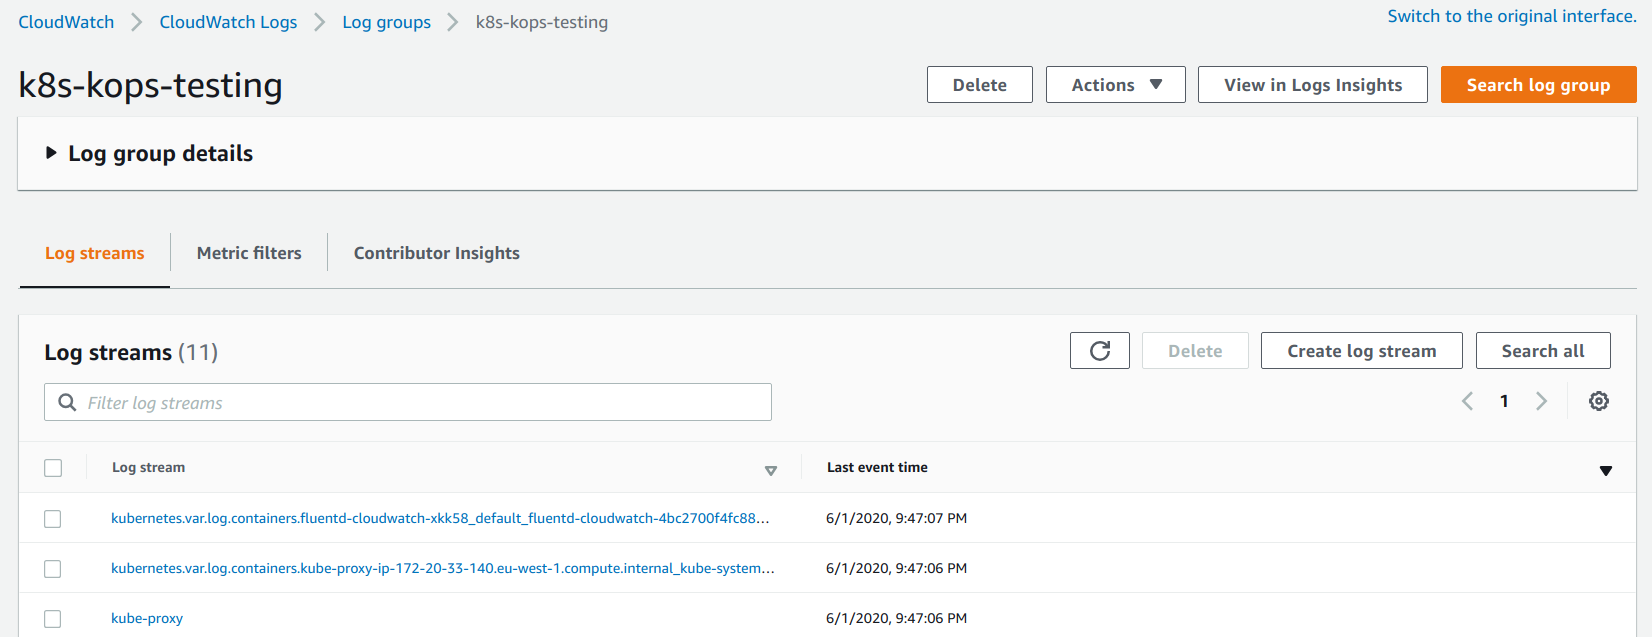
\includegraphics[width=16cm]{figures/kops-testing-cw-logs.png}
    \captionsetup{justification=centering,margin=2cm}
    \caption{AWS CloudWatch with logs from a Kubernetes cluster}}
\end{figure}
\begin{figure}[H]
    \centering
    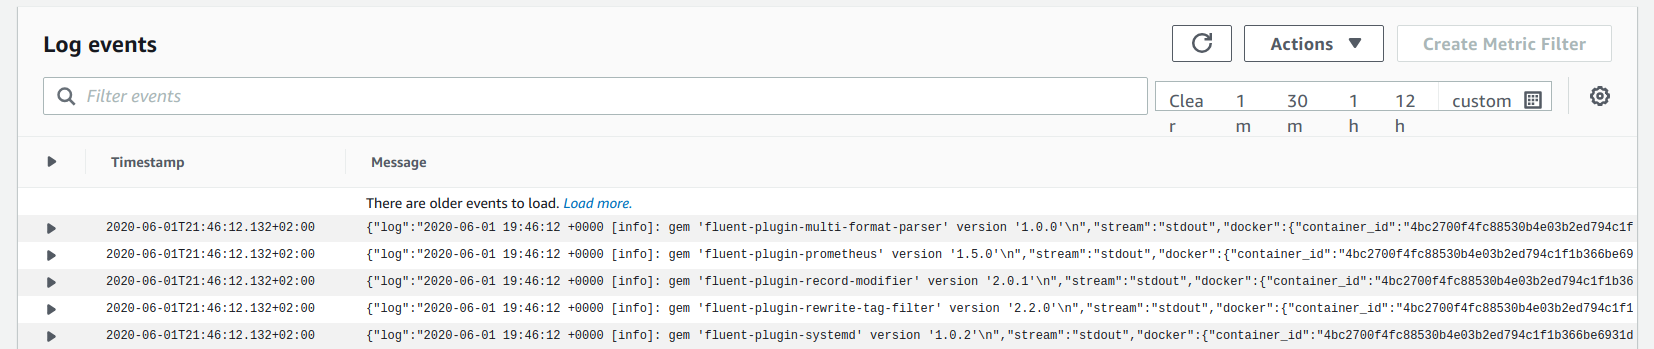
\includegraphics[width=16cm]{figures/kops-testing-cw-logs2.png}
    \captionsetup{justification=centering,margin=2cm}
    \caption{AWS CloudWatch with logs from a Kubernetes cluster}}
\end{figure}

An example log message looks like this:
\begin{lstlisting}[basicstyle=\tiny,caption={An example Kubernetes log message, presented on AWS CloudWatch},captionpos=b,language=Bash,xleftmargin=1cm]
{
    "log": "2020-06-01 19:46:12 +0000 [info]: gem 'fluent-plugin-multi-format-parser' version '1.0.0'\n",
    "stream": "stdout",
    "docker": {
        "container_id": "4bc2700f4fc88530b4e03b2ed794c1f1b366be6931d8500a8ccf21503d2c5b97"
    },
    "kubernetes": {
        "container_name": "fluentd-cloudwatch",
        "namespace_name": "default",
        "pod_name": "fluentd-cloudwatch-xkk58",
        "container_image": "fluent/fluentd-kubernetes-daemonset:v1.7.3-debian-cloudwatch-1.0",
        "container_image_id": "docker-pullable://fluent/fluentd-kubernetes-daemonset@sha256:9b8b2f99ea884853205150364eceaac9fff5ea97fc3300cc0080f48c3eac8b8a",
        "pod_id": "9fc38bd1-ff7b-4d29-9593-15796a7e5f94",
        "host": "ip-172-20-33-140.eu-west-1.compute.internal",
        "labels": {
            "app": "fluentd-cloudwatch",
            "controller-revision-hash": "68f7dc7cc",
            "pod-template-generation": "1",
            "release": "fluentd-cloudwatch"
        },
        "master_url": "https://100.64.0.1:443/api",
        "namespace_id": "4044bfd2-e836-43a1-bda1-71da0e985b9a"
    }
}
\end{lstlisting}

All the deployed Kubernetes components are listed below:
\begin{lstlisting}[basicstyle=\tiny,caption={TODO},captionpos=b,language=Bash,xleftmargin=1cm]
$ kubectl get -n kube-system pods
NAME                                                                READY   STATUS    RESTARTS   AGE
dns-controller-776cdf4ff4-lzb8f                                     1/1     Running   0          2m28s
etcd-manager-events-ip-172-20-39-5.eu-west-1.compute.internal       1/1     Running   0          2m20s
etcd-manager-main-ip-172-20-39-5.eu-west-1.compute.internal         1/1     Running   0          2m24s
kops-controller-49hsh                                               1/1     Running   0          89s
kube-apiserver-ip-172-20-39-5.eu-west-1.compute.internal            1/1     Running   3          82s
kube-controller-manager-ip-172-20-39-5.eu-west-1.compute.internal   1/1     Running   0          100s
kube-dns-autoscaler-594dcb44b5-7psf9                                1/1     Running   0          2m31s
kube-dns-b84c667f4-4wvsx                                            3/3     Running   0          2m32s
kube-dns-b84c667f4-kgdgb                                            3/3     Running   0          61s
kube-proxy-ip-172-20-39-5.eu-west-1.compute.internal                1/1     Running   0          2m20s
kube-scheduler-ip-172-20-39-5.eu-west-1.compute.internal            1/1     Running   0          93s
\end{lstlisting}

It can be also verified, that the custom labels applied to AWS resources by the cluster YAML configuration file, are indeed visible. The custom label here is: \textit{deployment: kops-testing}.
\begin{figure}[H]
    \centering
    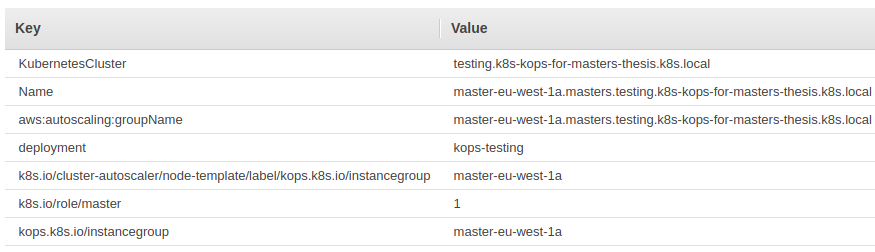
\includegraphics[width=16cm]{figures/kops-master-ec2-custom-tags.png}
    \captionsetup{justification=centering,margin=2cm}
    \caption{TODO}}
\end{figure}

When it comes to monitoring the cluster resources, some metrics are available by default on AWS EC2 dashboard. The information concerning CPU utilization or incoming network quantity in bytes can be viewed without any additional configuration. The example charts are depicted below.
\begin{figure}[H]
    \centering
    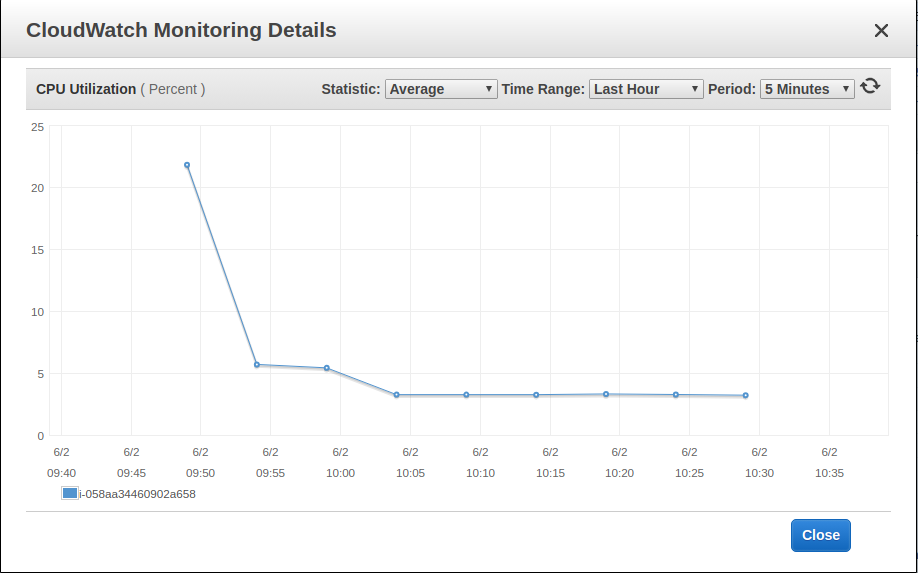
\includegraphics[width=13cm]{figures/k8s-kops-metrics-node1.png}
    \captionsetup{justification=centering,margin=2cm}
    \caption{TODO}}
\end{figure}
\begin{figure}[H]
    \centering
    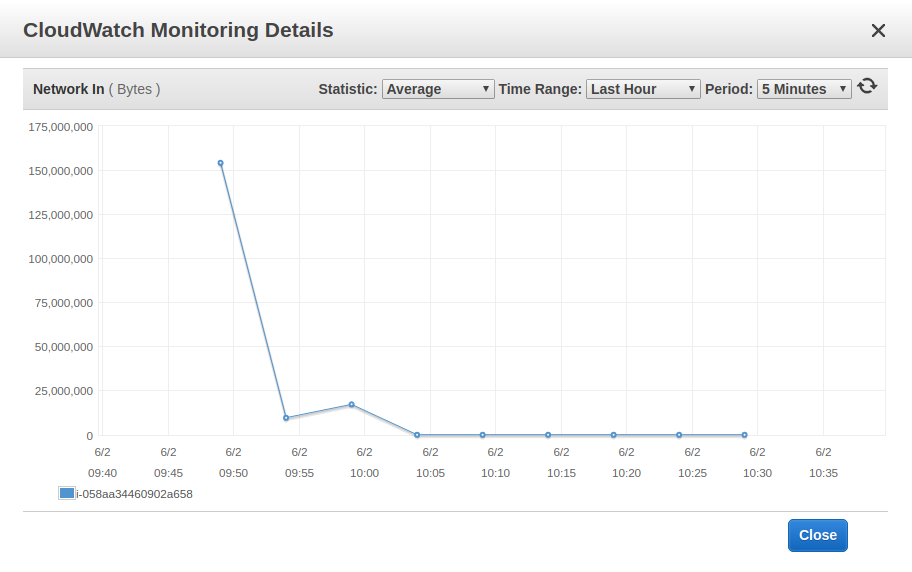
\includegraphics[width=13cm]{figures/k8s-kops-metrics-node2.png}
    \captionsetup{justification=centering,margin=2cm}
    \caption{TODO}}
\end{figure}

However, the above metrics concern only AWS resources metrics. An attempt to deploy a Kubernetes dashboard\cite{online-kops-addons} was made. That attempt was unsuccessful. First, a recommended command was run, which should have deployed the Kubernetes dashboard, but it resulted in an error:
\begin{lstlisting}[basicstyle=\tiny,caption={TODO},captionpos=b,language=Bash,xleftmargin=1cm]
$ kubectl create -f https://raw.githubusercontent.com/kubernetes/kops/master/addons/kubernetes-dashboard/v1.10.1.yaml
error: unable to recognize "https://raw.githubusercontent.com/kubernetes/kops/master/addons/kubernetes-dashboard/v1.10.1.yaml": no matches for kind "Deployment" in version "apps/v1beta2"
\end{lstlisting}

A very similar problem can be found among issues on github\cite{online-kops-dashboard-issue}. But, a newer version (2.0.1) of Kubernetes dashboard resources were found, thanks to a Github Pull Request\cite{online-kops-dashboard-issue-pr}. Deploying them resulted in two pods with status: Running.
\begin{lstlisting}[basicstyle=\tiny,caption={TODO},captionpos=b,language=Bash,xleftmargin=1cm]
$ $ kubectl get -n kubernetes-dashboard pod
NAME                                        READY   STATUS    RESTARTS   AGE
dashboard-metrics-scraper-c79c65bb7-cvd9r   1/1     Running   0          85s
kubernetes-dashboard-6f89967466-st5kw       1/1     Running   0          85s
\end{lstlisting}

However, there was a problem with accessing the dashboard in a web browser. Several ways have been tried (e.g. with trying Kubernetes resouce: Service with type: ClusterIP and NodePort, with running \textit{kubectl proxy}), but in result, deploying Kubernetes dashboard on a kops created cluster was unsuccessful.

When it comes to \textbf{Central Audit} requirement, no manual steps were needed. One can just log into AWS Management Console through a web browser, go to the AWS CloudTrail service and view the events history. Each event can be viewed and in return, information in JSON format is received. A table with events is presented on the picture below.

\begin{figure}[H]
    \centering
    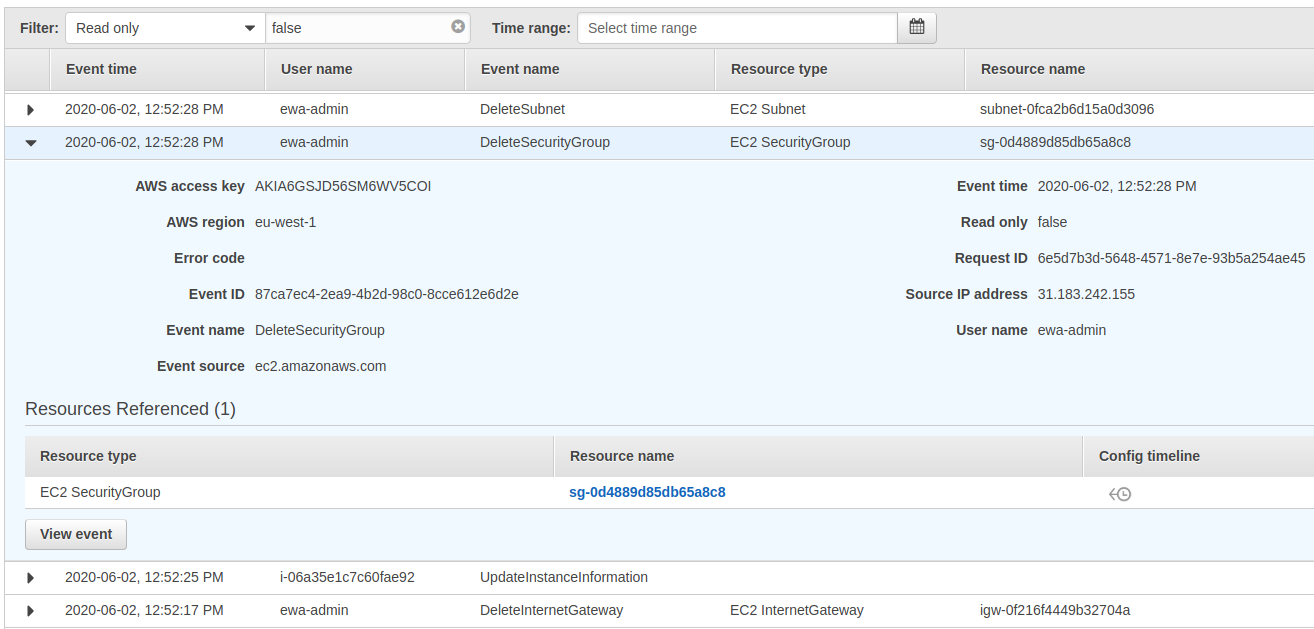
\includegraphics[width=13cm]{figures/kops-cloudtrail.png}
    \captionsetup{justification=centering,margin=2cm}
    \caption{TODO}}
\end{figure}

The next operation is to backup a cluster namespace. Velero was chosen as an application to facilitate backup. In order to install Velero CLI, one can run:
\begin{lstlisting}[basicstyle=\tiny,caption={TODO},captionpos=b,language=Bash,xleftmargin=1cm]
$ ./kops/tasks _install_velero_cli
\end{lstlisting}

The above command installed Velero client. A Velero Server must be also deployed on a Kubernetes cluster. Before it is done, AWS IAM user must be created and proper permissions must be assigned to it. The instructions how to deal with AWS IAM for Velero were available at Github\cite{velero-aws-plugin}. In order to be able to repeat the steps easily, all the instructions were saved to a Bash script as: \textit{src/velero/generate-velero-credentials.sh}. Running it should result in generating two credentials and exporting them as two Bash environment variable: \textit{$VELERO\_ACCESS\_KEY\_ID$} and \textit{$VELERO\_SECRET\_ACCESS\_KEY$}. Then, a file \textit{src/velero/credentials-velero} of such contents was created:
\begin{lstlisting}[basicstyle=\tiny,caption={TODO},captionpos=b,language=Bash,xleftmargin=1cm]
[default]
aws_access_key_id=<REPLACE-ME-WITH-SECRET>
aws_secret_access_key=<REPLACE-ME-WITH-SECRET>
\end{lstlisting}

Afterwards, a Velero Server was deployed, using a Helm chart. The following command was used:

\begin{lstlisting}[basicstyle=\tiny,caption={TODO},captionpos=b,language=Bash,xleftmargin=1cm]
$ kubectl create namespace velero
$ helm repo add vmware-tanzu https://vmware-tanzu.github.io/helm-charts
$ helm install velero --namespace velero -f velero-chart-values.yaml \
--set configuration.backupStorageLocation.bucket=${K8S_EXP_KOPS_S3_BUCKET} \
--set configuration.backupStorageLocation.prefix=${K8S_EXP_ENVIRONMENT} \
--set configuration.backupStorageLocation.config.region=${K8S_EXP_REGION} \
--set-file credentials.secretContents.cloud=${PWD}/../velero/credentials-velero \
--wait --atomic vmware-tanzu/velero
\end{lstlisting}

Then, a backup location for Velero was configured. It was done with the following command:
\begin{lstlisting}[basicstyle=\tiny,caption={TODO},captionpos=b,language=Bash,xleftmargin=1cm]
$ velero backup-location create default \
  --provider aws \
  --bucket ${K8S_EXP_KOPS_S3_BUCKET} \
  --prefix ${K8S_EXP_ENVIRONMENT} \
  --config region=${K8S_EXP_REGION}
Backup storage location "default" configured successfully.
\end{lstlisting}

And then, finally, the steps from Velero documentation was followed\cite{velero-examples}. A test application (provided by Velero) was deployed and backuped. The test application was deployed to a Kubernetes namespace: \textit{nginx-example}.   It was verified also that the Kubernetes resources were created.
\begin{lstlisting}[basicstyle=\tiny,caption={TODO},captionpos=b,language=Bash,xleftmargin=1cm]
$ kubectl apply -f velero-example.yaml
namespace/nginx-example created
deployment.apps/nginx-deployment created
service/my-nginx created
$ kubectl get -n nginx-example all
NAME                                    READY   STATUS              RESTARTS   AGE
pod/nginx-deployment-7cd5ddccc7-9drfn   1/1     Running   0          26s
pod/nginx-deployment-7cd5ddccc7-hr9zg   1/1     Running             0          7s

NAME               TYPE           CLUSTER-IP      EXTERNAL-IP                                                               PORT(S)        AGE
service/my-nginx   LoadBalancer   100.64.170.74   a64fbc3f7b55c45aead4f113025d8a34-1346547608.eu-west-1.elb.amazonaws.com   80:31927/TCP   7s

NAME                               READY   UP-TO-DATE   AVAILABLE   AGE
deployment.apps/nginx-deployment   1/2     2            1           7s

NAME                                          DESIRED   CURRENT   READY   AGE
replicaset.apps/nginx-deployment-7cd5ddccc7   2         2         1       8s
$ velero backup create nginx-backup1 --include-namespaces nginx-example
Backup request "nginx-backup1" submitted successfully.
Run `velero backup describe nginx-backup1` or `velero backup logs nginx-backup1` for more details.
$ velero backup describe nginx-backup1
Name:         nginx-backup1
# output partially ommitted
Phase:  Completed
$ velero backup logs nginx-backup1
# output partially ommitted
time="2020-06-03T13:35:51Z" level=info msg="Backed up a total of 24 items" backup=velero/nginx-backup1 logSource="pkg/backup/backup.go:436" progress=
\end{lstlisting}

The backup result was stored in an S3 bucket and it is presented in the image below:
\begin{figure}[H]
    \centering
    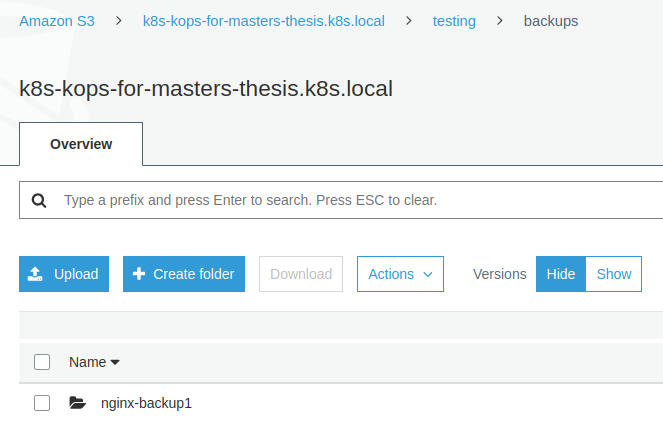
\includegraphics[width=10cm]{figures/kops-velero-backup.png}
    \captionsetup{justification=centering,margin=2cm}
    \caption{Backup of a Kubernetes namespace created by Velero, kept in an S3 bucket}}
\end{figure}

Next, a disaster was simulated. The whole \textit{nginx-example} namespace was deleted:
\begin{lstlisting}[basicstyle=\tiny,caption={TODO},captionpos=b,language=Bash,xleftmargin=1cm]
$ kubectl delete namespaces nginx-example
namespace "nginx-example" deleted
$ kubectl get -n nginx-example all
No resources found in nginx-example namespace.
\end{lstlisting}

The last step was to restore the namespace from Velero backup. It was successful.
\begin{lstlisting}[basicstyle=\tiny,caption={TODO},captionpos=b,language=Bash,xleftmargin=1cm]
$ velero restore create --from-backup nginx-backup1
Restore request "nginx-backup1-20200603133811" submitted successfully.
Run `velero restore describe nginx-backup1-20200603133811` or `velero restore logs nginx-backup1-20200603133811` for more details.
$ kubectl get -n nginx-example all
NAME                                    READY   STATUS    RESTARTS   AGE
pod/nginx-deployment-7cd5ddccc7-9drfn   1/1     Running   0          9s
pod/nginx-deployment-7cd5ddccc7-hr9zg   1/1     Running   0          8s

NAME               TYPE           CLUSTER-IP      EXTERNAL-IP                                                               PORT(S)        AGE
service/my-nginx   LoadBalancer   100.71.21.114   abf6080d1d43a43ba97999bb6b22cabc-2114878664.eu-west-1.elb.amazonaws.com   80:32539/TCP   8s

NAME                               READY   UP-TO-DATE   AVAILABLE   AGE
deployment.apps/nginx-deployment   2/2     2            2           8s

NAME                                          DESIRED   CURRENT   READY   AGE
replicaset.apps/nginx-deployment-7cd5ddccc7   2         2         2       8s
\end{lstlisting}


Then, autoscaling was tested. The autoscaler Kubernetes resources were deployed with:
\begin{lstlisting}[basicstyle=\tiny,caption={TODO},captionpos=b,language=Bash,xleftmargin=1cm]
kops$ ./tasks _enable_as
\end{lstlisting}
which basically just deployed the resources configured at autoscaler git repository\cite{as-github}. Some modifications were also applied to the cluster YAML configuration, namely: under \textit{additionalPolicies} of node configuration, the following code was added:
\begin{lstlisting}[basicstyle=\tiny,caption={TODO},captionpos=b,language=Bash,xleftmargin=1cm]
{
  "Effect": "Allow",
  "Action": [
    "autoscaling:DescribeAutoScalingGroups",
    "autoscaling:DescribeAutoScalingInstances",
    "autoscaling:DescribeLaunchConfigurations",
    "autoscaling:SetDesiredCapacity",
    "autoscaling:TerminateInstanceInAutoScalingGroup",
    "autoscaling:DescribeTags"
  ],
  "Resource": "*"
}
\end{lstlisting}
Also, additional labels for InstanceGroup of worker nodes were set and maximum number of worker nodes were set to 2. This went smoothly thanks to a blog post\cite{as-blog}. The modified configuration is presented below:
\begin{lstlisting}[basicstyle=\tiny,caption={TODO},captionpos=b,language=Bash,xleftmargin=1cm]
spec:
  cloudLabels:
    service: k8s_node
    k8s.io/cluster-autoscaler/enabled: ""
    k8s.io/cluster-autoscaler/testing.k8s-kops-for-masters-thesis.k8s.local: ""
  minSize: 1
  maxSize: 2
\end{lstlisting}

In order to test the autoscaling, a test application was deployed with:
\begin{lstlisting}[basicstyle=\tiny,caption={TODO},captionpos=b,language=Bash,xleftmargin=1cm]
tests$ ./deploy-test-service.sh
\end{lstlisting}
After the above command ended with success, it was verified that 1 pod replica was deployed. Since, the task here was to make the autoscaler decide to scale out - to add another node, the test application deployment was scaled, so that 200 pod replicas were deployed.
\begin{lstlisting}[basicstyle=\tiny,caption={TODO},captionpos=b,language=Bash,xleftmargin=1cm]
kops$ kubectl get -n testing deployment
NAME             READY   UP-TO-DATE   AVAILABLE   AGE
apache-testing   1/1     1            1           9m48s
kops$ kubectl scale -n testing deployment apache-testing --replicas=200
deployment.apps/apache-testing scaled
kops$ kubectl get -n testing deployment
NAME             READY    UP-TO-DATE   AVAILABLE   AGE
apache-testing   12/200   200          12        13m
\end{lstlisting}
This triggered the creation of another node and in a short while, there were two nodes in the cluster:
\begin{lstlisting}[basicstyle=\tiny,caption={TODO},captionpos=b,language=Bash,xleftmargin=1cm]
kops$ aws ec2 describe-instances --filters "Name=tag-key,Values=deployment" --query "Reservations[*].Instances[*].{PublicIP:PublicIpAddress,Name:Tags[?Key=='Name']|[0].Value,Status:State.Name}"
[
    [
        {
            "PublicIP": "34.242.4.10",
            "Name": "master-eu-west-1a.masters.testing.k8s-kops-for-masters-thesis.k8s.local",
            "Status": "running"
        }
    ],
    [
        {
            "PublicIP": "34.247.37.124",
            "Name": "nodes.testing.k8s-kops-for-masters-thesis.k8s.local",
            "Status": "running"
        }
    ],
    [
        {
            "PublicIP": "3.249.123.18",
            "Name": "nodes.testing.k8s-kops-for-masters-thesis.k8s.local",
            "Status": "running"
        }
    ]
]
\end{lstlisting}
Afterwards, the pod replicas were scaled back to 1 and then, autoscaler terminated one of the worker nodes. Soon, one of the EC2 instances was in the status: terminated. This proved that autoscaler works for a Kubernetes cluster deployed with kops.

When it comes to running a cluster in the High Availability mode, there were no problems whatsoever. No matter if the cluster was created with one master node or multiple master nodes - it was working. In HA mode, the following was returned as information about the cluster:
\begin{lstlisting}[basicstyle=\tiny,caption={TODO},captionpos=b,language=Bash,xleftmargin=1cm]
$ kubectl get nodes
NAME                                          STATUS   ROLES    AGE   VERSION
ip-172-20-108-29.eu-west-1.compute.internal   Ready    master   73s   v1.16.9
ip-172-20-55-72.eu-west-1.compute.internal    Ready    node     49s   v1.16.9
ip-172-20-61-242.eu-west-1.compute.internal   Ready    master   74s   v1.16.9
ip-172-20-89-96.eu-west-1.compute.internal    Ready    master   75s   v1.16.9
$ kops validate
Validating cluster testing.k8s-kops-for-masters-thesis.k8s.local

INSTANCE GROUPS
NAME			ROLE	MACHINETYPE	MIN	MAX	SUBNETS
master-eu-west-1a	Master	t2.micro	1	1	eu-west-1a
master-eu-west-1b	Master	t2.micro	1	1	eu-west-1b
master-eu-west-1c	Master	t2.micro	1	1	eu-west-1c
nodes			Node	t2.micro	1	1	eu-west-1a

NODE STATUS
NAME						ROLE	READY
ip-172-20-108-29.eu-west-1.compute.internal	master	True
ip-172-20-55-72.eu-west-1.compute.internal	node	True
ip-172-20-61-242.eu-west-1.compute.internal	master	True
ip-172-20-89-96.eu-west-1.compute.internal	master	True

Your cluster testing.k8s-kops-for-masters-thesis.k8s.local is ready
\end{lstlisting}

The machines can be also viewed on AWS Management Console:
\begin{figure}[H]
    \centering
    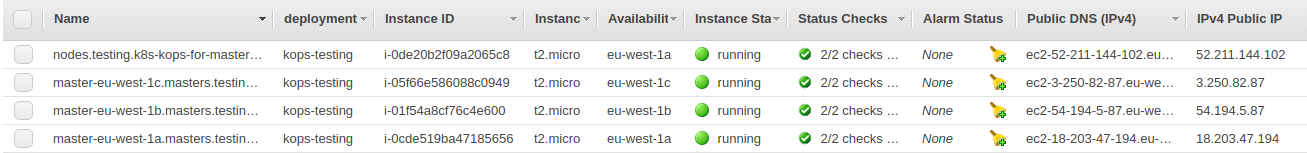
\includegraphics[width=18cm]{figures/k8s-kops-ha-aws.png}
    \captionsetup{justification=centering,margin=2cm}
    \caption{TODO}}
\end{figure}

Also, the tests were invoked both in HA mode and also with one master cluster. The tests succeeded in both cases. In HA mode, all the Kubernetes control plane components were duplicated (in this case - three times):
\begin{lstlisting}[basicstyle=\tiny,caption={TODO},captionpos=b,language=Bash,xleftmargin=1cm]
$ kubectl -n kube-system get pod
NAME                                                                  READY   STATUS    RESTARTS   AGE
dns-controller-776cdf4ff4-xw4tg                                       1/1     Running   0          2m18s
etcd-manager-events-ip-172-20-108-29.eu-west-1.compute.internal       1/1     Running   0          66s
etcd-manager-events-ip-172-20-61-242.eu-west-1.compute.internal       1/1     Running   0          86s
etcd-manager-events-ip-172-20-89-96.eu-west-1.compute.internal        1/1     Running   0          96s
etcd-manager-main-ip-172-20-108-29.eu-west-1.compute.internal         1/1     Running   0          53s
etcd-manager-main-ip-172-20-61-242.eu-west-1.compute.internal         1/1     Running   0          56s
etcd-manager-main-ip-172-20-89-96.eu-west-1.compute.internal          1/1     Running   0          80s
kops-controller-2tz4h                                                 1/1     Running   0          2m8s
kops-controller-7mr7s                                                 1/1     Running   0          2m14s
kops-controller-psfch                                                 1/1     Running   0          2m8s
kube-apiserver-ip-172-20-108-29.eu-west-1.compute.internal            1/1     Running   3          110s
kube-apiserver-ip-172-20-61-242.eu-west-1.compute.internal            1/1     Running   3          114s
kube-apiserver-ip-172-20-89-96.eu-west-1.compute.internal             1/1     Running   3          92s
kube-controller-manager-ip-172-20-108-29.eu-west-1.compute.internal   1/1     Running   0          2m6s
kube-controller-manager-ip-172-20-61-242.eu-west-1.compute.internal   1/1     Running   0          105s
kube-controller-manager-ip-172-20-89-96.eu-west-1.compute.internal    1/1     Running   0          79s
kube-dns-autoscaler-594dcb44b5-ccnjf                                  1/1     Running   0          2m19s
kube-dns-b84c667f4-5tb9z                                              3/3     Running   0          105s
kube-dns-b84c667f4-8vmh4                                              3/3     Running   0          2m21s
kube-proxy-ip-172-20-108-29.eu-west-1.compute.internal                1/1     Running   0          116s
kube-proxy-ip-172-20-55-72.eu-west-1.compute.internal                 1/1     Running   0          110s
kube-proxy-ip-172-20-61-242.eu-west-1.compute.internal                1/1     Running   0          65s
kube-proxy-ip-172-20-89-96.eu-west-1.compute.internal                 1/1     Running   0          61s
kube-scheduler-ip-172-20-108-29.eu-west-1.compute.internal            1/1     Running   0          2m
kube-scheduler-ip-172-20-61-242.eu-west-1.compute.internal            1/1     Running   0          2m13s
kube-scheduler-ip-172-20-89-96.eu-west-1.compute.internal             1/1     Running   0          112s
\end{lstlisting}

\subsubsection{Testing a cluster}
\label{testing-cluster}
All the tests can be invoked with a single command:
\begin{lstlisting}[basicstyle=\tiny,caption={TODO},captionpos=b,language=Bash,xleftmargin=1cm]
$ ./kops/tasks _test
\end{lstlisting}

This one command runs the following:
\begin{lstlisting}[basicstyle=\tiny,caption={TODO},captionpos=b,language=Bash,xleftmargin=1cm]
$ set -x
$ time kops validate cluster ${K8S_EXP_CLUSTER_NAME} --state "s3://${K8S_EXP_KOPS_S3_BUCKET}"
$ cd ../tests
$ time bats tests.bats
$ cd ../kops
\end{lstlisting}

The \textit{kops validate cluster} command is provided by the kops CLI. It checks that all k8s master and worker nodes are running and have "Ready" status, that all the components are healthy and that all pods in the kube-system namespace are running and healthy\cite{online-kops-valid}. The next command runs the Bats-core tests. They test the version of Kubernetes, number of worker nodes and also they deploy a test Helm chart with Apache Server. All the tests and the deployment (and later deletion) of the Apache Helm chart are automated and intended to be idempotent. Thanks to such a test, it is verified that such a Kubernetes cluster is ready to use for the end users.

The test Apache Server serves a very simple website, which all code is just one index.html file with the following contents:
\begin{lstlisting}[basicstyle=\tiny,caption={TODO},captionpos=b,language=Bash,xleftmargin=1cm]
<html>
<head>
<title>Hello world</title>
</head>
<body>
<p>Welcome to my Master Thesis website!</p>
</body>
</html>
\end{lstlisting}
Thus, there is a test that runs: \textit{curl} command and expects that the output contains "Welcome to my Master Thesis website!". Such a test is possible thanks to an ingress resource provided by the Apache Helm Chart. When this ingress is deployed on a Kubernetes cluster on AWS, an Elastic Load Balancer (ELB) is created. ELB is an AWS resource. The ELB provides us with the endpoint that can be used with \textit{curl}.

The tests were run with Bats-core and their code is presented below:
\begin{lstlisting}[basicstyle=\tiny,caption={TODO},captionpos=b,language=Bash,xleftmargin=1cm]
@test "kubernetes machines have correct version" {
  run /bin/bash -c "kubectl version | grep 'Server Version'"
  # this is printed on test failure only
  echo "# test cmd output: $output"
  [[ "${output}" =~ "v1.16" ]]
  [ "$status" -eq 0 ]
}

@test "1 kubernetes worker nodes have status: Ready" {
  run /bin/bash -c "chmod +x get-workers-count.sh && ./get-workers-count.sh"
  # this is printed on test failure only
  echo "# test cmd output: $output"
  [[ "${output}" =~ "1" ]]
  [ "$status" -eq 0 ]
}

@test "kubectl cluster-info returns expected output" {
  run /bin/bash -c "kubectl cluster-info"
  # this is printed on test failure only
  echo "# test cmd output: $output"
  [[ "${output}" =~ "Kubernetes master" ]]
  [[ "${output}" =~ "https://" ]]
  # this works for kops cluster only:
  # [[ "${output}" =~ "https://api-testing-k8s-kops-for" ]]
  # output for eks:
  # Kubernetes master is running at https://E1B139B821FFAEF37082A7B64BB951FC.gr7.eu-west-1.eks.amazonaws.com
  # CoreDNS is running at https://E1B139B821FFAEF37082A7B64BB951FC.gr7.eu-west-1.eks.amazonaws.com/api/v1/namespaces/kube-system/services/kube-dns:dns/proxy
  [ "$status" -eq 0 ]
}

@test "a test application can be deployed on kubernetes" {
  run /bin/bash -c "chmod +x ./deploy-test-service.sh && ./deploy-test-service.sh"
  # this is printed on test failure only
  echo "# test cmd output: $output"
  [[ "${output}" =~ "Success" ]]
  [ "$status" -eq 0 ]

  # k8s resource: pod was created
  run /bin/bash -c "kubectl get --namespace=testing pods"
  # this is printed on test failure only
  echo "# test cmd output: $output"
  [[ "${output}" =~ "apache-testing" ]]
  [[ "${output}" =~ "Running" ]]
  [ "$status" -eq 0 ]

  # k8s resource: svc was created
  run /bin/bash -c "kubectl get --namespace=testing svc"
  # this is printed on test failure only
  echo "# test cmd output: $output"
  [[ "${output}" =~ "apache-testing" ]]
  [ "$status" -eq 0 ]

  # k8s resource: ing was created
  run /bin/bash -c "kubectl get --namespace=testing ing"
  # this is printed on test failure only
  echo "# test cmd output: $output"
  [[ "${output}" =~ "apache-testing" ]]
  [ "$status" -eq 0 ]
}

@test "a test application is available (ingress resource works)" {
  # the LoadBalancer on AWS does not work right away, so here
  # we try it many times, until it works (max 400 trials)
  run /bin/bash -c "export SERVICE_IP=$(kubectl get svc --namespace testing apache-testing --template '{{ range (index .status.loadBalancer.ingress 0) }}{{.}}{{ end }}') && chmod +x test-timeout-until.sh && ./test-timeout-until.sh \"curl --max-time 2 -L http://\$SERVICE_IP 2>/dev/null | grep 'Welcome to my Master Thesis website'\" \"400\" \"curl --max-time 2 -L http://\$SERVICE_IP 2>/dev/null | grep 'Welcome to my Master Thesis website'\""
  # this is printed on test failure only
  echo "# test cmd output: $output"
  [[ "${output}" =~ "Welcome to my Master Thesis website" ]]
  [ "$status" -eq 0 ]
}

@test "a test service (test website) can be deleted from kubernetes" {
  run /bin/bash -c 'helm uninstall --namespace="testing" "apache-testing" && kubectl delete -f config-map-www-contents.yaml && kubectl delete namespace "testing"'
  echo "# test cmd output: $output"
  [[ "${output}" =~ "uninstalled" ]]
  [ "$status" -eq 0 ]

  # pod, svc and ing resources were deleted
  run /bin/bash -c 'kubectl get --namespace=testing pods,svc,ing'
  echo "# test cmd output: $output"
  [[ "${output}" =~ "No resources found in testing namespace" ]]
  [ "$status" -eq 0 ]
}
\end{lstlisting}
Several helpful scripts were created and used for the tests. All the needed files are put in the git repository on Github.com. TODO link


%%%

\subsubsection{Deleting a cluster}

\subsubsection{Troubleshooting}

\textbf{The first problem} was, that the command responsible for creating a cluster did not wait until the cluster was ready. It returned as soon as the AWS resources were scheduled for creation. This was a problem, because if one wanted to create, test and then delete a Kubernetes cluster in a CI pipeline, then the tests would never work. And the pipeline would always fail. The solution for this problem was already described in the section \ref{kops-creating-the-cluster}.

\textbf{The second problem} was how to configure logging to AWS CloudWatch. The documentation of the Helm chart: kube2iam\cite{kube2iam} provided an example command of how to deploy the chart: \textit{helm install stable/kube2iam --name my-release}. But this resulted in errors, which are presented below, thanks to debugging the kube2iam pod.
\begin{lstlisting}[basicstyle=\tiny,caption={TODO},captionpos=b,language=Bash,xleftmargin=1cm]
$ kubectl get pod
NAME                       READY   STATUS             RESTARTS   AGE
kube2iam-2c8vv             0/1     CrashLoopBackOff   9          17m
$ kubectl logs kube2iam-2c8vv
E0601 10:35:53.142224       1 reflector.go:199] github.com/jtblin/kube2iam/vendor/k8s.io/client-go/tools/cache/reflector.go:94: Failed to list *v1.Pod: pods is forbidden: User "system:serviceaccount:default:default" cannot list resource "pods" in API group "" at the cluster scope
E0601 10:35:53.142621       1 reflector.go:199] github.com/jtblin/kube2iam/vendor/k8s.io/client-go/tools/cache/reflector.go:94: Failed to list *v1.Namespace: namespaces is forbidden: User "system:serviceaccount:default:default" cannot list resource "namespaces" in API group "" at the cluster scope
\end{lstlisting}

These errors went away, when the chart was deployed with additional settings set: \textit{helm upgrade "kube2iam" --namespace="default" --wait --atomic --set rbac.create=true stable/kube2iam}.

\textbf{The third problem} concerned the lack of permissions of the fluentd-cloudwatch pod. It manifested in the following way:
\begin{lstlisting}[basicstyle=\tiny,caption={TODO},captionpos=b,language=Bash,xleftmargin=1cm]
$ kubectl logs fluentd-cloudwatch-xkk58
2020-06-01 11:03:14 +0000 [warn]: #0 [out_cloudwatch_logs_host_logs] failed to flush the buffer. retry_time=8 next_retry_seconds=2020-06-01 11:05:22 +0000 chunk="5a703b5e45c9592f24399f9b73acaf43" error_class=Aws::CloudWatchLogs::Errors::AccessDeniedException error="User: arn:aws:sts::976184668068:assumed-role/nodes.testing.k8s-kops-for-masters-thesis.k8s.local/i-04a926040234f36d6 is not authorized to perform: logs:DescribeLogGroups on resource: arn:aws:logs:eu-west-1:976184668068:log-group::log-stream:"
\end{lstlisting}
This problem was also already dealt with in the section \ref{kops-creating-the-cluster}. The solution was to add IAM permissions in the YAML template configuration file. The solution was inspired by a Tobias Sturm's blog post\cite{kops-logs-cw-tobias} and by the kops documentation\cite{online-kops-iam}.

\textbf{The fourth problem} was with testing the Apache Server. The essential thing to know is that it takes some time (around 5 minutes) for the ELB to be usable by end users and thus the tests may fail in the meantime. The solution was to implement such a command that verifies the Apache Server endpoint many times, but has a maximum number of trials.

There were also \textbf{problems with deploying Velero}. For example, using the example deployment command provided on the Velero Helm Chart page on Github.com vmware-tanzu\cite{velero-helm-chart}, but omitting the aws plugin for Velero resulted in error.

\begin{lstlisting}[basicstyle=\tiny,caption={TODO},captionpos=b,language=Bash,xleftmargin=1cm]
$ helm repo add vmware-tanzu https://vmware-tanzu.github.io/helm-charts
# output omitted
$ helm install velero --namespace default \
  --set configuration.provider=aws \
  --set configuration.backupStorageLocation.name=aws \
  --set configuration.backupStorageLocation.bucket=${K8S_EXP_KOPS_S3_BUCKET} \
  --set configuration.backupStorageLocation.prefix=${K8S_EXP_ENVIRONMENT} \
  --set configuration.backupStorageLocation.config.region=${K8S_EXP_REGION} \
  --wait --atomic \
  vmware-tanzu/velero
# output omitted
$ kubectl logs -n default velero-7f476777f6-f9qlc
An error occurred: some backup storage locations are invalid: error getting backup store for location "aws": unable to locate ObjectStore plugin named velero.io/aws
\end{lstlisting}

Tinkering with that command resulted also in different error:
\begin{lstlisting}[basicstyle=\tiny,caption={TODO},captionpos=b,language=Bash,xleftmargin=1cm]
Error: release velero failed, and has been uninstalled due to atomic being set: timed out waiting for the condition
\end{lstlisting}

It was then decided to try another command to install Velero server. It pushed the progress further and revealed the problem:
\begin{lstlisting}[basicstyle=\tiny,caption={TODO},captionpos=b,language=Bash,xleftmargin=1cm]
$  velero install \
    --provider velero.io/aws \
    --bucket ${K8S_EXP_KOPS_S3_BUCKET} \
    --plugins velero/velero-plugin-for-aws:v1.1.0 \
    --backup-location-config s3Url=${K8S_EXP_KOPS_S3_BUCKET},region=${K8S_EXP_REGION} \
    --use-volume-snapshots=false \
    --secret-file=${PWD}/credentials-velero
Velero is installed! ⛵ Use 'kubectl logs deployment/velero -n velero' to view the status.
$ kubectl get -n velero all
NAME                          READY   STATUS    RESTARTS   AGE
pod/velero-5f8889f694-6xd7t   0/1     Pending   0          2m30s

NAME                     READY   UP-TO-DATE   AVAILABLE   AGE
deployment.apps/velero   0/1     1            0           2m30s

NAME                                DESIRED   CURRENT   READY   AGE
replicaset.apps/velero-5f8889f694   1         1         0       2m30s
$ kubectl -n velero describe pods
Name:           velero-5f8889f694-6xd7t
Namespace:      velero
Limits:
     cpu:     1
     memory:  256Mi
   Requests:
     cpu:     500m
     memory:  128Mi
Warning  FailedScheduling  70s (x5 over 6m46s)  default-scheduler  0/2 nodes are available: 2 Insufficient cpu.
\end{lstlisting}

The problem was that the Velero pod was in status: Pending. The Kubernetes documentation on pods troubleshooting suggests, that when a pod is in status: Pending, then there may be not enough resources in the cluster\cite{k8s-deb}. That was the problem in this case. The solution was to use bigger AWS instance types for node: \textit{t2.medium} instead of: \textit{t2.micro}.

A \textbf{problem considering autoscaler deployment} was observed. The Kubernetes resources provided by the official git repository on Github.com had a minor mistake. The autoscaler pod was in error state and it returned the following error:
\begin{lstlisting}[basicstyle=\tiny,caption={TODO},captionpos=b,language=Bash,xleftmargin=1cm]
$ kubectl describe -n kube-system pod/cluster-autoscaler-8b46dddf5-8xkns
Warning  Failed     26s                kubelet, ip-172-20-62-245.eu-west-1.compute.internal  Error: failed to start container "cluster-autoscaler": Error response from daemon: OCI runtime create failed: container_linux.go:346: starting container process caused "process_linux.go:449: container init caused \"rootfs_linux.go:58: mounting \\\"/etc/ssl/certs/ca-bundle.crt\\\" to rootfs \\\"/var/lib/docker/overlay2/0f99e6ea6c9a9f8dedf87b977b72ecff7b56e0e6e439fcd8f9275bda3dbcabe6/merged\\\" at \\\"/var/lib/docker/overlay2/0f99e6ea6c9a9f8dedf87b977b72ecff7b56e0e6e439fcd8f9275bda3dbcabe6/merged/etc/ssl/certs/ca-certificates.crt\\\" caused \\\"not a directory\\\"\"": unknown: Are you trying to mount a directory onto a file (or vice-versa)? Check if the specified host path exists and is the expected type
Warning  BackOff    12s (x2 over 42s)  kubelet, ip-172-20-62-245.eu-west-1.compute.internal  Back-off restarting failed container
\end{lstlisting}

Fortunately, this problem was handled by a public issue and the solution was also provided there\cite{as-github-issue}. The solution was to replace a path: \textit{/etc/ssl/certs/ca-certificates.crt} with \textbf{/etc/ssl/certs/ca-bundle.crt}.



\subsection{Production deployment using eksctl}
\textit{This section briefly presents all the steps performed that lead to a Kubernetes cluster deployment on the AWS cloud using eksctl. Here an attempt was made to satisfy all the production environment requirements selected in the chapter: \ref{prep-prod}.}
\\

\subsubsection{Generating the YAML configuration file}
When using eksctl, it is possible to create a cluster with \textit{eksctl create cluster} command and either with setting command line options or with using a YAML file. The latter solution was chosen. In contrast to kops, it was easier to create such YAML file by hand. Due to the fact that it was desired to automate the cluster deployment across multiple environments, it was decided that there will be one configuration file named: \textit{cluster.tmpl.yaml}. This file will contain Bash variables as some values. This file will be used as a template. Then, to create a configuration file for production environment, such commands were run:
\begin{lstlisting}[basicstyle=\tiny,caption={TODO},captionpos=b,language=Bash,xleftmargin=1cm]
export K8S_EXP_REGION="eu-west-1"
export K8S_EXP_ENVIRONMENT="production"
export K8S_EXP_CLUSTER_NAME="eks-${K8S_EXP_ENVIRONMENT}"
my_ip=$(curl https://ipinfo.io/ip 2>/dev/null)
sed "s/\${K8S_EXP_CLUSTER_NAME}/${K8S_EXP_CLUSTER_NAME}/" cluster.tmpl.yaml > cluster1.yaml
sed "s/\${K8S_EXP_REGION}/${K8S_EXP_REGION}/" cluster1.yaml > cluster2.yaml
sed "s/\${K8S_EXP_ENVIRONMENT}/${K8S_EXP_ENVIRONMENT}/" cluster2.yaml > cluster3.yaml
sed "s'\${my_ip}'${my_ip}/32'" cluster3.yaml > cluster.yaml
rm cluster1.yaml cluster2.yaml cluster3.yaml
time eksctl create cluster -f cluster.yaml
\end{lstlisting}

All these commands were scripted and thanks to the automation, they can be invoked just by running:
\begin{lstlisting}[basicstyle=\tiny,caption={TODO},captionpos=b,language=Bash,xleftmargin=1cm]
eks$ ./tasks _create
\end{lstlisting}
This command creates a configuration file for a particular environment and then it deploys a Kubernetes cluster. The whole \textit{cluster.tmpl.yaml} file is presented below:
\begin{lstlisting}[basicstyle=\tiny,caption={TODO},captionpos=b,language=Bash,xleftmargin=1cm]
apiVersion: eksctl.io/v1alpha5
kind: ClusterConfig

metadata:
  name: eks-testing
  region: eu-west-1
  version: "1.16"
  tags:
    deployment: eks-testing

cloudWatch:
  clusterLogging:
    enableTypes: ["api", "audit", "authenticator", "controllerManager", "scheduler"]

nodeGroups:
  - name: ng-1
    labels: { role: worker, cluster: eks-testing }
    instanceType: t2.nano
    desiredCapacity: 1
    ssh:
      allow: true

\end{lstlisting}

Thanks to \textit{metadata.tags} set in the YAML file, the AWS resources were labeled with a custom tag: \textit{deployment: eks-testing} or \textit{deployment: eks-production} (depending on the environment). Below there are images of a CloudFormation and EKS resource with tags, viewed on AWS Management Console.
\begin{figure}[H]
    \centering
    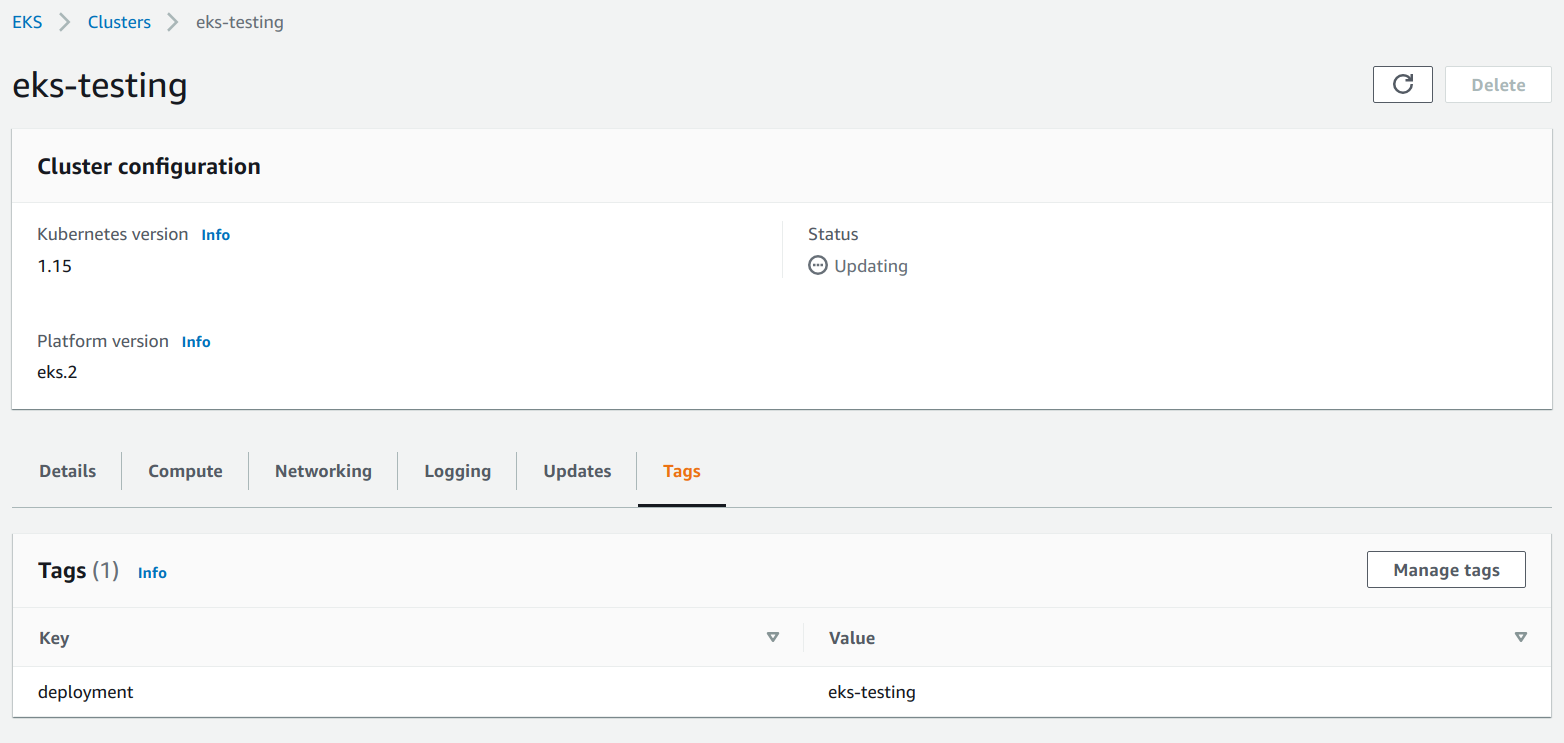
\includegraphics[width=16cm]{figures/eks-on-aws-mc-tags.png}
    \captionsetup{justification=centering,margin=2cm}
    \caption{AWS EKS resource with tags set, viewed on AWS Management Console}}
\end{figure}
\begin{figure}[H]
    \centering
    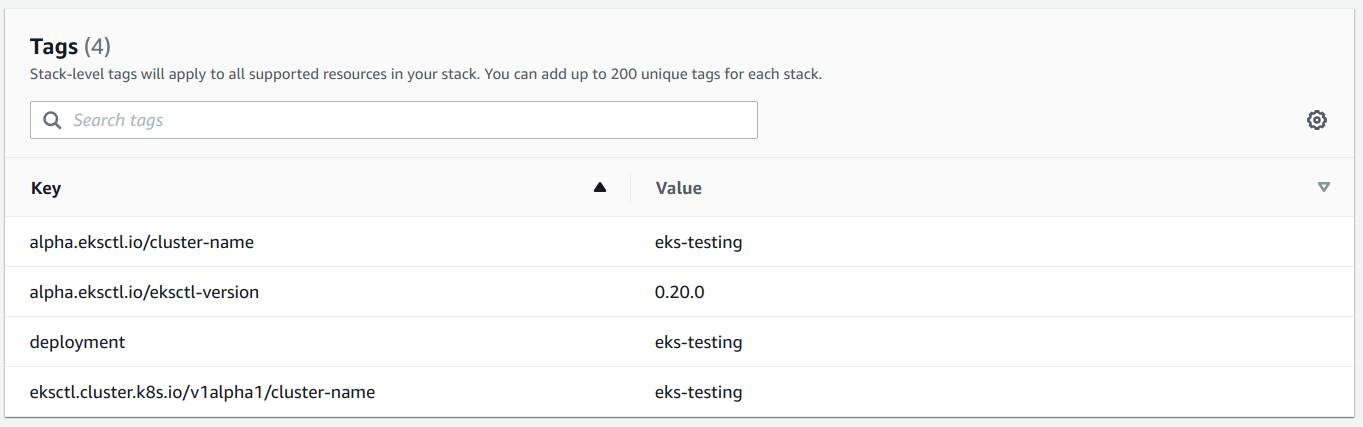
\includegraphics[width=16cm]{figures/eks-cf-tags.png}
    \captionsetup{justification=centering,margin=2cm}
    \caption{AWS CloudFormation resource with tags set, viewed on AWS Management Console}}
\end{figure}

\subsubsection{Creating the cluster}
There was one command used to generate cluster configuration (described in the previous section) and to deploy the cluster. The nice thing from the end user point of view was, that this command did not return (meaning: it waited) for the cluster to be ready. First, the control plane was deployed, then the worker nodes. For each of these two tasks (deploying control plane and deploying worker nodes) a separate CloudFormation stack was used. It was done automatically by AWS EKS. The image below presents such two stacks.

\begin{figure}[H]
    \centering
    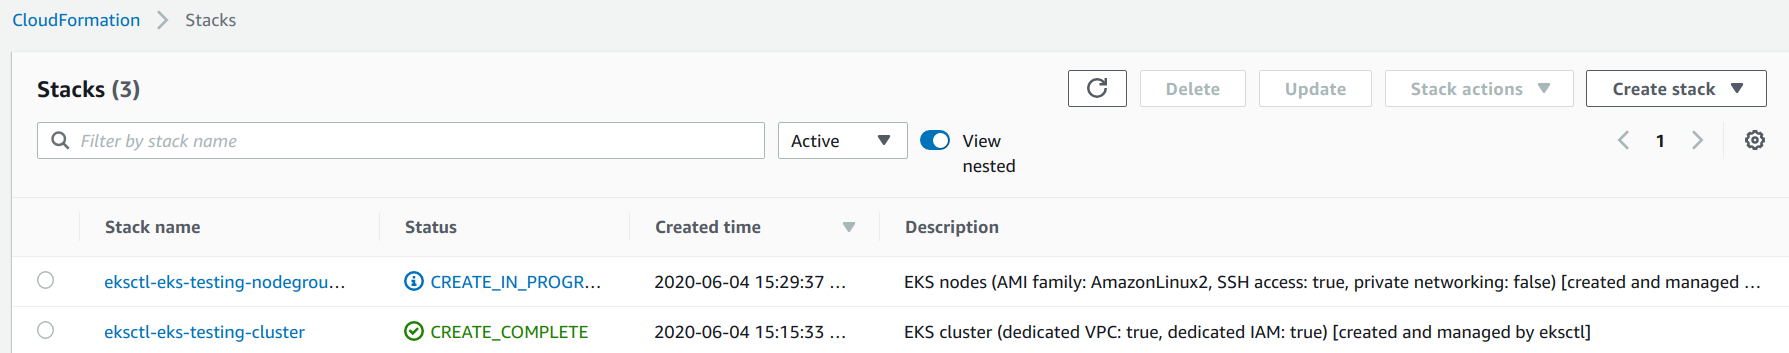
\includegraphics[width=16cm]{figures/eks-cf-stacks.png}
    \captionsetup{justification=centering,margin=2cm}
    \caption{TODO}}
\end{figure}

It was also possible to view the AWS resources which were provided by each CloudFormation stack. It is illustrated below.
\begin{figure}[H]
    \centering
    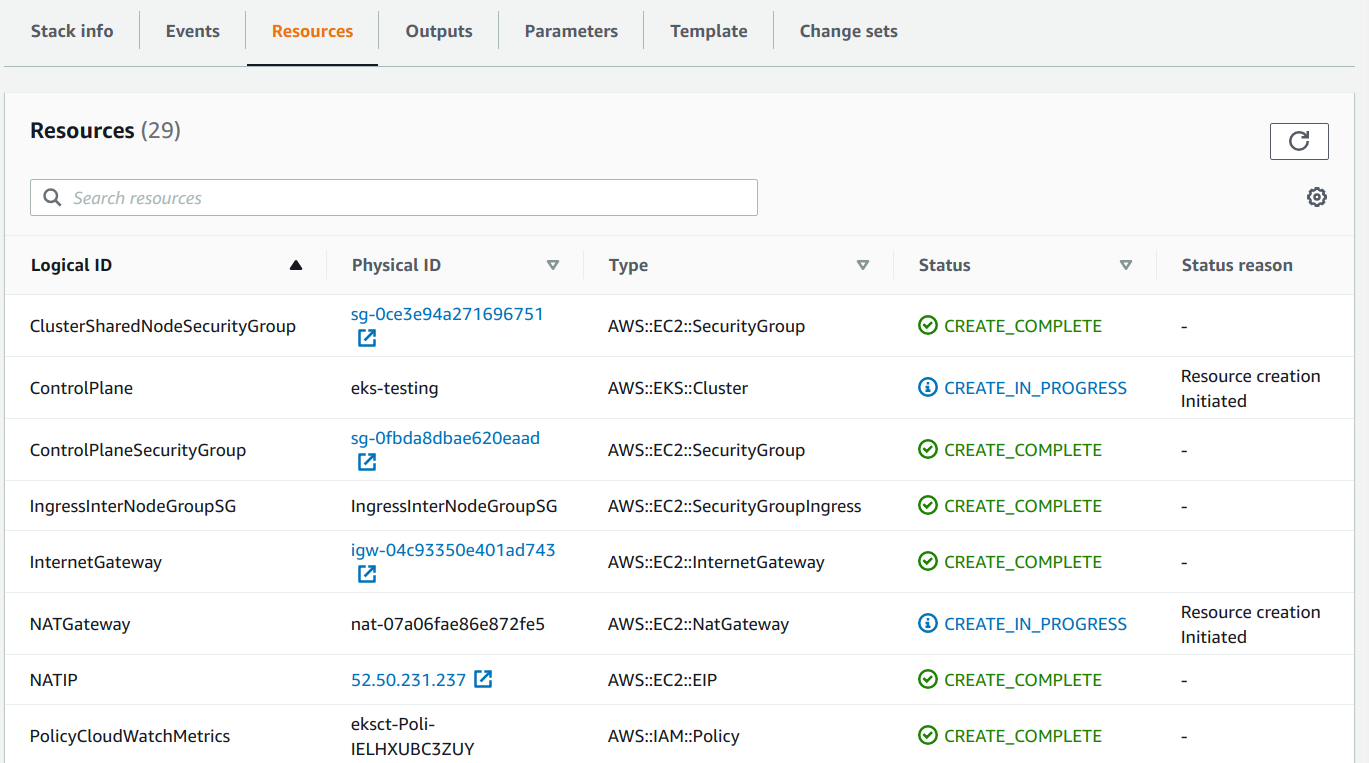
\includegraphics[width=16cm]{figures/eks-cf-resources.png}
    \captionsetup{justification=centering,margin=2cm}
    \caption{TODO}}
\end{figure}

The control plane is entirely managed by AWS and it is run across three AWS availability zones in order to ensure high availability. The end user has even no access to the control plane, meaning: there is no EC2 instance with master node visible and when listing all Kubernetes nodes, only the worker nodes are visible.
\begin{figure}[H]
    \centering
    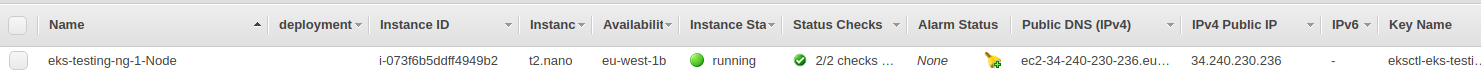
\includegraphics[width=16cm]{figures/eks-on-aws-node.png}
    \captionsetup{justification=centering,margin=2cm}
    \caption{TODO}}
\end{figure}

A few sources claimed that the creation of Kubernetes cluster on AWS EKS should take 10 - 15 minutes\cite{eks-blog-part1}\cite{eks-blog2}, but in this particular case it took about 20 minutes. Also, to the best of this work’s author knowledge, there was no command which allows to reconfigure the cluster. This means that when there was a need to change e.g. tags of the AWS resources, the cluster must have been deleted and created from scratch. An issue on Github.com was created to acknowledge this problem\cite{eksctl-no-config-update}. There is, however, a command that enables to upgrade the control plane to the next Kubernetes version (if it available). This command is:
\begin{lstlisting}[basicstyle=\tiny,caption={TODO},captionpos=b,language=Bash,xleftmargin=1cm]
$ eksctl update cluster
\end{lstlisting}

Enabling the Central Logging was very easy. All what was needed was adding the following code to the configuration YAML file:
\begin{lstlisting}[basicstyle=\tiny,caption={TODO},captionpos=b,language=Bash,xleftmargin=1cm]
cloudWatch:
  clusterLogging:
    enableTypes: ["api", "audit", "authenticator", "controllerManager", "scheduler"]
\end{lstlisting}

In result, an AWS LogGroup was created and all the log messages from Kubernetes components were directed onto the LogGroup.

\begin{figure}[H]
    \centering
    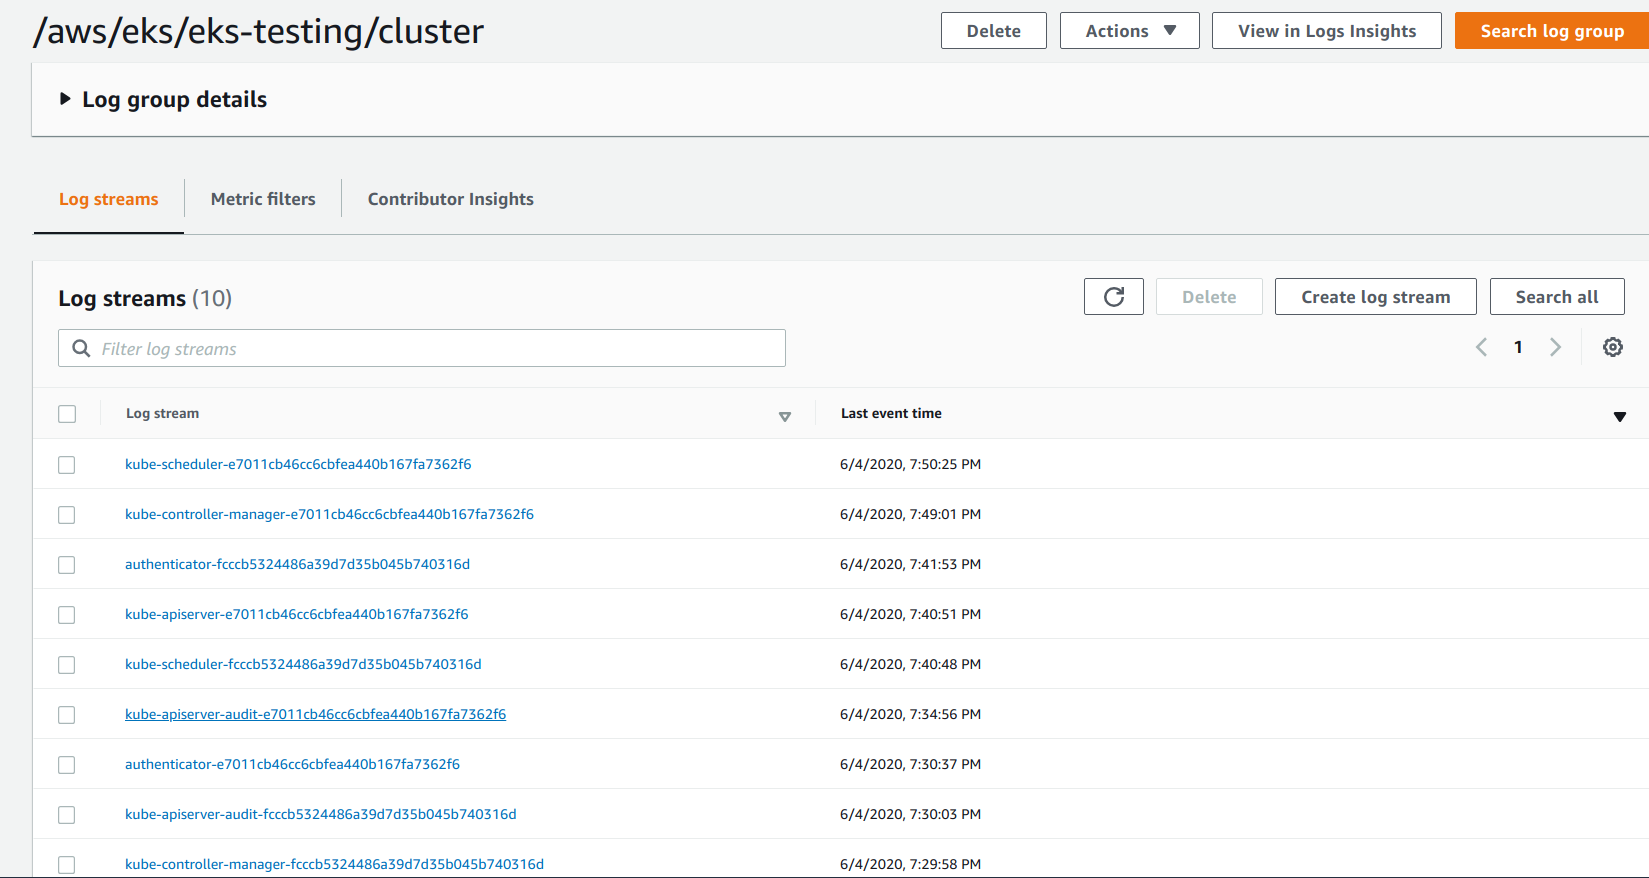
\includegraphics[width=16cm]{figures/eks-cw.png}
    \captionsetup{justification=centering,margin=2cm}
    \caption{TODO}}
\end{figure}
\begin{figure}[H]
    \centering
    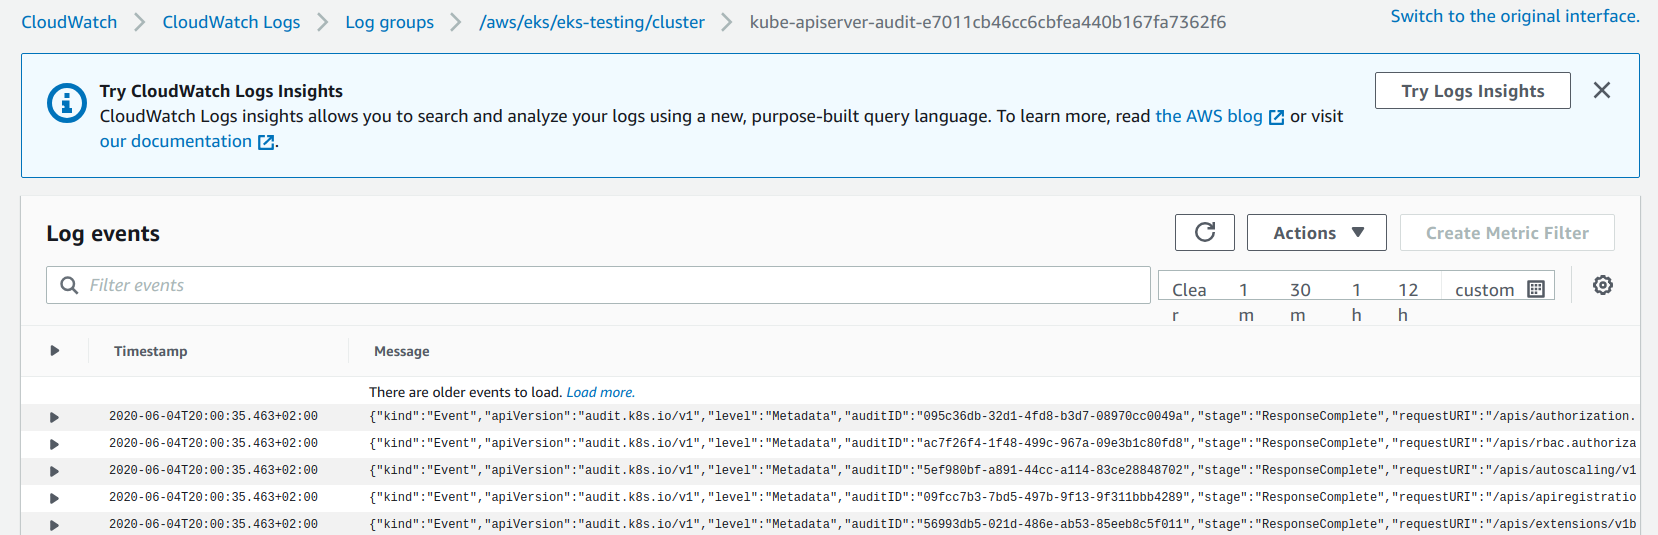
\includegraphics[width=16cm]{figures/eks-cw-apiserver.png}
    \captionsetup{justification=centering,margin=2cm}
    \caption{TODO}}
\end{figure}

An example log message looked like this and it was in JSON format:

\begin{lstlisting}[basicstyle=\tiny,caption={TODO},captionpos=b,language=Bash,xleftmargin=1cm]
2020-06-04T20:00:36.463+02:00
{
    "kind": "Event",
    "apiVersion": "audit.k8s.io/v1",
    "level": "Metadata",
    "auditID": "454b8586-2d17-4a53-9eb5-1e7422aabd21",
    "stage": "ResponseComplete",
    "requestURI": "/api?timeout=32s",
    "verb": "get",
    "user": {
        "username": "system:serviceaccount:kube-system:resourcequota-controller",
        "uid": "b7f3c725-196f-4b25-94e4-8f75614d3a04",
        "groups": [
            "system:serviceaccounts",
            "system:serviceaccounts:kube-system",
            "system:authenticated"
        ]
    },
    "sourceIPs": [
        "10.0.162.1"
    ],
    "userAgent": "kube-controller-manager/v1.16.8 (linux/amd64) kubernetes/e163110/system:serviceaccount:kube-system:resourcequota-controller",
    "responseStatus": {
        "metadata": {},
        "code": 200
    },
    "requestReceivedTimestamp": "2020-06-04T18:00:36.279592Z",
    "stageTimestamp": "2020-06-04T18:00:36.279722Z",
    "annotations": {
        "authorization.k8s.io/decision": "allow",
        "authorization.k8s.io/reason": "RBAC: allowed by ClusterRoleBinding \"system:discovery\" of ClusterRole \"system:discovery\" to Group \"system:authenticated\""
    }
}
\end{lstlisting}

There was nothing needed to be done in order to provide High Availability. The control plane was already Highly Available because AWS EKS automatically provisions and scales the control plane across multiple AWS availability zones for high availability and fault tolerance\cite{eks-faqs}. Even the output provided when creating the cluster confirms the HA:
\begin{lstlisting}[basicstyle=\tiny,caption={TODO},captionpos=b,language=Bash,xleftmargin=1cm]
+ eksctl create cluster -f cluster.yaml
[ℹ]  eksctl version 0.20.0
[ℹ]  using region eu-west-1
[ℹ]  setting availability zones to [eu-west-1a eu-west-1b eu-west-1c]
[ℹ]  subnets for eu-west-1a - public:192.168.0.0/19 private:192.168.96.0/19
[ℹ]  subnets for eu-west-1b - public:192.168.32.0/19 private:192.168.128.0/19
[ℹ]  subnets for eu-west-1c - public:192.168.64.0/19 private:192.168.160.0/19
\end{lstlisting}

When it comes to Central Audit, also no additional steps were taken. The actions performed on AWS resources are automatically visible on AWS CloudTrail dashboard. This is the same case as with kops. Since both methods use AWS, they both utilize CloudTrail. An example view showing the CloudTrail events, which occurred due to deleting an EKS cluster is shown next.
\begin{figure}[H]
    \centering
    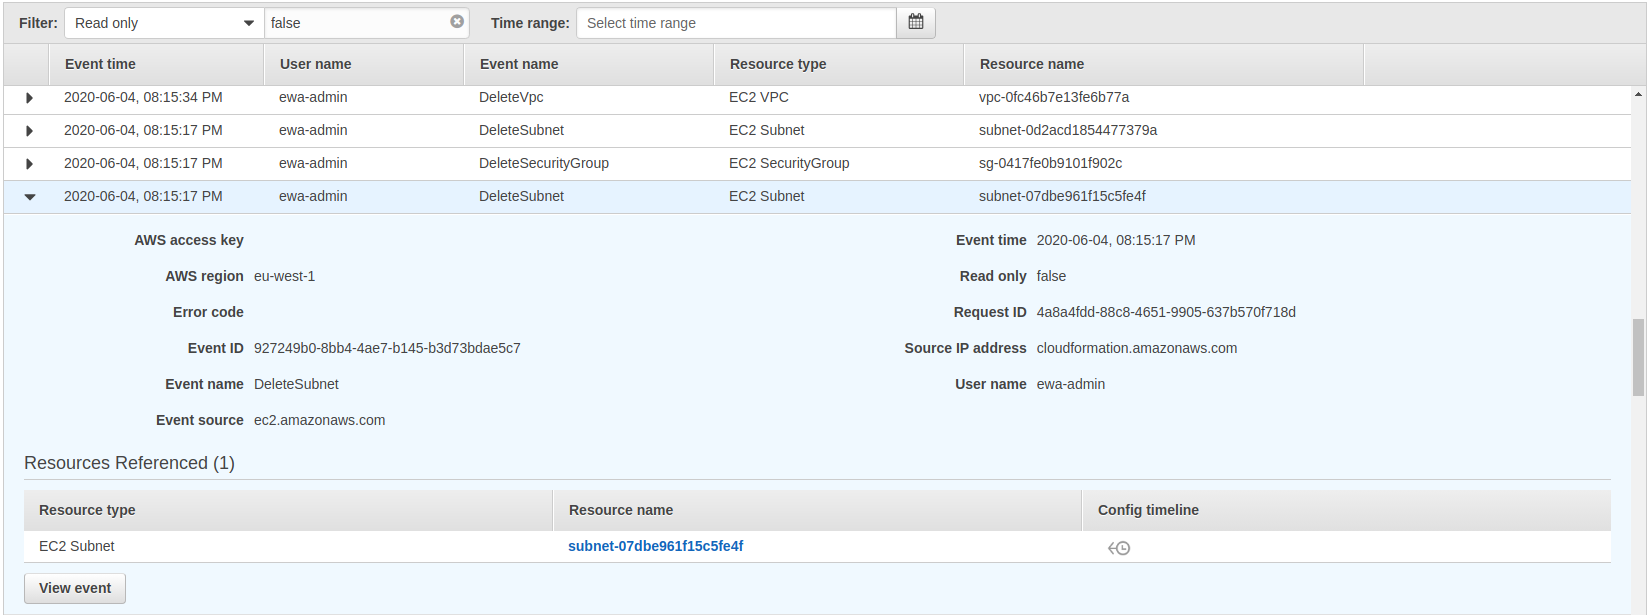
\includegraphics[width=17cm]{figures/eks-ct.png}
    \captionsetup{justification=centering,margin=2cm}
    \caption{TODO}}
\end{figure}


todo: kubectl get -n kube-system pods

\subsubsection{Testing the cluster}
The testing procedure was the same as with kops. Different command was invoked (because all the commands to run with eksctl were put into one file), but all the Bats-core tests were the same. Even the same bats files were used. There was obviously no \textit{kops validate cluster} command run, because that command was dedicated to kops clusters only. For the details, please refer to \ref{Testing a cluster}. Running all the tests took slightly less than 7 minutes. (It took long to have a working Load Balancer). The command to run tests was:
\begin{lstlisting}[basicstyle=\tiny,caption={TODO},captionpos=b,language=Bash,xleftmargin=1cm]
eks$ ./tasks _test
\end{lstlisting}

\subsubsection{Deleting the cluster}
In order to delete the cluster, one had to type:
\begin{lstlisting}[basicstyle=\tiny,caption={TODO},captionpos=b,language=Bash,xleftmargin=1cm]
eks$ ./tasks _delete
\end{lstlisting}

This command usually took about 13 minutes. It deleted almost all AWS resources, but not CloudWatch LogGroup. Not deleting the LogGroup may be a good thing, because one may be interested to study the logs after the cluster is long gone. But still, it is good to know, that one has to delete it by themselves.

\subsubsection{Troubleshooting the cluster}
The greatest problem was how to set some security measures. Setting the following in the YAML configuration file:

\begin{lstlisting}[basicstyle=\tiny,caption={TODO},captionpos=b,language=Bash,xleftmargin=1cm]
vpc:
  publicAccessCIDRs:
    - "31.183.242.155/32"
\end{lstlisting}
resulted in timeout on creating such cluster. It took 43 minutes then. The output ended with:

\begin{lstlisting}[basicstyle=\tiny,caption={TODO},captionpos=b,language=Bash,xleftmargin=1cm]
[ℹ]  adding identity "arn:aws:iam::976184668068:role/eksctl-eks-testing-nodegroup-ng-1-NodeInstanceRole-8VB5IDO1Z4KQ" to auth ConfigMap
[ℹ]  nodegroup "ng-1" has 0 node(s)
[ℹ]  waiting for at least 1 node(s) to become ready in "ng-1"
Error: timed out (after 25m0s) waiting for at least 1 nodes to join the cluster and become ready in "ng-1"
\end{lstlisting}


```
[ℹ]  waiting for at least 1 node(s) to become ready in "ng-1"

^C
dojo@88999332cb7d(k8s-aws-dojo):/dojo/work/eks$ eksctl update cluster -f cluster.yaml
[ℹ]  eksctl version 0.20.0
[ℹ]  using region eu-west-1
[!]  NOTE: config file is used for finding cluster name and region
[!]  NOTE: cluster VPC (subnets, routing & NAT Gateway) configuration changes are not yet implemented
[ℹ]  re-building cluster stack "eksctl-eks-testing-cluster"
[✔]  all resources in cluster stack "eksctl-eks-testing-cluster" are up-to-date
[ℹ]  checking security group configuration for all nodegroups
[ℹ]  all nodegroups have up-to-date configuration
dojo@88999332cb7d(k8s-aws-dojo):/dojo/work/eks$ kubectl get nodes
No resources found in default namespace.
```

%%

troubleshooting k8s -mastering k8s p. 58 cite{k8s-deb}
* what happens if we manually delete a iptables rule? kube-proxy will put it back after 10 to 30s - https://learnk8s.io/blog/kubernetes-chaos-engineering-lessons-learned
* https://learnk8s.io/troubleshooting-deployments - must read!!
